%!TEX TS-program = xelatex
%!TEX encoding = UTF-8

% LaTeX source for book ``代数学方法'' in Chinese
% Copyright 2018  李文威 (Wen-Wei Li).
% Permission is granted to copy, distribute and/or modify this
% document under the terms of the Creative Commons
% Attribution 4.0 International (CC BY 4.0)
% http://creativecommons.org/licenses/by/4.0/

% 《代数学方法》卷一: 基础结构 / 李文威
% 使用自定义的文档类 AJbook.cls. 自动载入 xeCJK. 需要额外档案如下:
% font-setup-HEP.tex/font-setup-open.tex, coverpage.tex, titles-setup.tex, mycommand.sty, myarrows.sty
% 文档类选项 (key/val 格式):
% mydraft = true (未定稿, 底部显示日期) 或 false (成品), 默认 false,
% mycolors = true (链接带颜色无框) 或 false (黑色无框), 默认 true,
% coverpage = 封面档档名, 默认为空 (此时不制作封面), 若为 *.pdf 的形式则直接引入 PDF 页面.
% fontsetup = 字体设置档档名,
% titlesetup = 章节格式设置档名.

% 需动用 imakeidx + xindy (两份索引), biblatex + biber (书目). 
% 索引用土法进行中文排序: 如 \index{zhongwen@中文} 等.
\documentclass[
%	draftmark = true,
	colors = true,
%	colors = false,
	coverpage = coverpage.tex,
%	coverpage = coverpage.pdf,
	fontsetup = font-setup-open.tex,
%	fontsetup = font-setup-HEP.tex,
	titlesetup = titles-setup.tex
]{AJbook}

\usepackage{mathrsfs}
\usepackage{stmaryrd} \SetSymbolFont{stmry}{bold}{U}{stmry}{m}{n}	% 避免警告 (stmryd 不含粗体故)
\usepackage{array}
\usepackage{makecell}	% 便于制表
\usepackage{tikz-cd}  % 使用 TikZ 绘图
\usetikzlibrary{positioning, patterns, calc, matrix, shapes.arrows, shapes.symbols}
\usepackage{braids}
\usepackage{tqft}
\usepackage{ytableau}

% PGF plots 用于封面绘制
\usepackage{pgfplots}
\pgfplotsset{compat=newest}

% 设置章节深度
%\setcounter{secnumdepth}{1}

% 必要时仅引入部分档案
% \includeonly{}

\usepackage{myarrows}				% 使用自定义的可伸缩箭头
\usepackage{mycommand}				% 引入自定义的惯用的命令

% 生成索引: 选用 xindy + imakeidx
\usepackage[xindy, splitindex]{imakeidx}
\makeindex[
	columns=2,
	program=truexindy,
	intoc=true,
	options=-M texindy -I xelatex -C utf8,
	title={名词索引暨英译}]	% 名词索引
\makeindex[
	columns=3,
	program=truexindy,
	intoc=true,
	options=-M numeric-sort -M latex -M latex-loc-fmts -M makeindex -I xelatex -C utf8,
	name=sym1,
	title={符号索引}]	% 符号索引

\usepackage[unicode, bookmarksnumbered]{hyperref}	% 启动超链接和 PDF 文档信息所需
% 设置 PDF 文件信息
\hypersetup{
	pdfauthor = {杨鼎 (Ding Yang)},
	pdftitle = {随机过程回顾},
	pdfkeywords = {Algebra},
	CJKbookmarks = true}

% 用 bibLaTeX 生成参考文献
% 载入书目库: 文档类业已引入 biblatex + biber
\addbibresource{Al-jabr.bib}

\begin{document}
\frontmatter	% 制作封面和目录.

\mainmatter		% 正文开始:逐章引入 TeX 代码

% LaTeX source for book ``代数学方法'' in Chinese
% Copyright 2018  李文威 (Wen-Wei Li).
% Permission is granted to copy, distribute and/or modify this
% document under the terms of the Creative Commons
% Attribution 4.0 International (CC BY 4.0)
% http://creativecommons.org/licenses/by/4.0/

% To be included
\chapter*{导言}	% 文档类会自动将之加入目录并设置天眉

首先分享几条清华大学张颢老师的几条格言:
\begin{itemize}
	\item No Reading, No Learning.参考多本教程或教材可以让你理解更深刻,但\textbf{一定}要找一个教程深入学习,其他作为参考和辅助。大量的阅读是学习的重要内容。
	\item No Writing, No Reading(Effective Reading).把读到的每个符号都在纸上写一遍。
	\item No Data, No Truth.所有的模型都是人造的,只有数据是上帝给的,数据才是对真理最无私的反映。
	\item No Analytic, No Understanding.一件事在解析上算不清楚就不叫真正理解。
	\item No Programing, No Cognition.理解停留在上层,而认知需要落地。
\end{itemize}

根据费曼学习法,将学到的知识讲述出来可以加深自己的理解,同时也是一个重新整理思路的过程,这是整理这篇文档的初衷。文档中的定义、定理和证明等内容为求准确,完全与《应用随机过程(第6版)》内容一致;文字描述少部分参照教材中描述,大多数是个人的理解,所以难免有偏差;习题选自教材例题和习题(龙汉:我建议大家关注),留出了很多空白,需要动手去完成。

本文档\LaTeX 模板来自北京大学数学科学学院李文威老师《代数学方法》(\href{https://github.com/wenweili/AlJabr-1}{GitHub链接}),节约了很多精力,在此作出感谢。 \nopagebreak

\vspace{1em}
\begin{flushright}\begin{minipage}{0.3 \textwidth}
		\begin{tabular}{c}
			{\kaishu 杨鼎} \\
			2024 年 5 月于北斗楼309
		\end{tabular}
	\end{minipage}\end{flushright}
\vspace{1em}


% LaTeX source for book ``代数学方法'' in Chinese
% Copyright 2018  李文威 (Wen-Wei Li).
% Permission is granted to copy, distribute and/or modify this
% document under the terms of the Creative Commons
% Attribution 4.0 International (CC BY 4.0)
% http://creativecommons.org/licenses/by/4.0/

% To be included
\chapter{随机过程概述}

\begin{compactitem}
	\item 概率空间、随机变量、随机过程.
	\item 分布函数与概度函数.
	\item 均值函数、方差函数、协方差函数、自相关函数、特征函数.
	\item 独立增量过程、平稳增量过程、严格平稳过程与广义(宽)平稳过程.
\end{compactitem}

\section{随机变量}\label{sec:RandomVar}

\begin{definition}\label{def:prob-space}\index{gailvkongjian@概率空间 (probability space)}
	设\((\Omega,\mathscr{F})\)是可测空间,\(P(\cdot)\)是定义在\(\mathscr{F}\)上的实值函数。如果
	\begin{enumerate}[\bfseries (1)]
		\item \(P(\Omega)=1\),
		\item \(\forall A\in \mathscr{F},0\leq P(A)\leq 1\),
		\item 对两两互不相容事件\(A_1,A_2,A_3,\dots\)(即当\(i\neq j\)时,\(A_i \cap A_j\neq \varnothing\) ).
	\end{enumerate}
	有\begin{align*}
		P\left(\bigcup_{i=1}^{\infty} A_i\right)=\sum_{i=1}^{\infty}P(A_i)
	\end{align*}
	则称P是\((\Omega,\mathscr{F})\)上的\emph{概率},\(\Omega,\mathscr{F},P\)称为\emph{概率空间},
	\(\mathscr{F}\)中的元素称为事件,P(A)称为事件A的概率。
\end{definition}


\begin{definition}\label{def:RV-CDF}\index{suijibianliang@随机变量 (random variable)}\index{fenbuhanshu@分布函数 (cumulative distribution function)}
	设\((\Omega,\mathscr{F},P)\)是(完备的)概率空间,X是定义在上取值于实数集的函数,
	如果\(\forall x \in \mathbb{R} , \{w : X(\omega)\leqslant x\}\in \mathscr{F}\),
	则称X是\(\mathscr{F}\)上的随机变量,简称\emph{随机变量}。函数
	\begin{align*}
		F(x)=P\{\omega:X(\omega)\leqslant x\},\quad -\infty<x<\infty
	\end{align*}
	称为随机变量X的\emph{分布函数}。
\end{definition}

注意到,随机变量是定义在概率空间和实数集之间的函数(映射)。\emph{随机变量}中,\emph{随机}指的是事件在概率空间中随机发生,\emph{变量}指的是事件对应的函数值,这种对应关系(即函数)是确定的。

实际中常用的随机变量有两种类型:离散型随机变量和连续性随机变量。

离散型随机变量X的概率分布用如下分布列来描述:
\begin{align*}
	p_k=P\{X=x_k\},\quad k=1,2,\dots
\end{align*}
其分布函数为:
\begin{align*}
	F(x)=\sum_{x_k\leqslant x}p_k
\end{align*}

连续型随机变量X的概率分布用概率密度函数\(f(x)\)描述,其分布函数为:
\begin{align*}
	F(x)=\int_{-\infty}^{x}f(t)dt
\end{align*}
对于随机向量\(\mathbf{X}=(X_1,X_2,\dots,X_d)\),它的联合分布函数定义为:
\begin{align*}
	F(x_1,x_2,\dots,x_d)=P\{X_1\leqslant x_1,X_2\leqslant x_2,\dots,X_d\leqslant x_d\}
\end{align*}
这里\(d\geqslant 1,x_k\in \mathbb{R}\ (k=1,2,\dots ,d)\)。

\begin{definition}\label{def:num-feat}\index{shuzitezheng@随机变量的数字特征(number features)}
	\begin{enumerate}[\bfseries (1)]
		\item 取值为\({s_k}\)的离散型随机变量的\emph{数学期望}定义为:
		      \begin{align*}
			      E(X)=\sum_{k}s_k P\{X=s_k\}=\sum_{k}s_k p_k
		      \end{align*}
		      如果\(\sum\left\lvert s_k\right\rvert p_k<+\infty\)。
		\item 连续型随机变量X的\emph{数学期望}定义为:
		      \begin{align*}
			      E(X)=\int_{-\infty}^{\infty}xdF(x)=\int_{-\infty}^{\infty}xf(x)dx
		      \end{align*}
		      如果\(\int_{-\infty}^{\infty} \left\lvert x\right\rvert dF(x)<+\infty\)。
		      这里,\(F(x)\)是X的分布函数,\(f(x)\)是其密度函数。

		      利用Riemann-Stieltjes积分,可以对离散型随机变量和连续性随机变量的期望给出一个统一的表达式:
		      \begin{align*}
			      E(X)=\int_{-\infty}^{+\infty}xdF(x)
		      \end{align*}
		\item 设X为随机变量,若\(E[X-E(x)]^2\)存在,则称\(E[X-E(x)]^2\)为X的\emph{方差},记为Var(X),即\(Var(x)=\int_{-\infty}^{+\infty}[X-E(x)]^2dF(x)\)。
		\item 对两个随机变量X,Y,若\(E\{[X-E(X)][Y-E(Y)]\}\)存在,则称之为X与Y的\emph{协方差},记为Cov(X,Y),可知\(Cov(X,Y)=E(XY)-E(X)E(Y)\)。
		\item 设X为任一随机变量,对正整数k,称\(c_k=E[X-E(X)]^k\)为X的k阶\emph{中心矩}。方差是二阶中心矩。
		\item 设X,Y为两个随机变量,对正整数k,l,称\(E[X-E(X)]^k[Y-E(Y)]^l\)为X和Y的的k+l阶\emph{混合中心矩}。协方差是二阶混合中心矩。
	\end{enumerate}
\end{definition}

\begin{definition}\label{def:MomGengun-CharFun}\index{jumuhanshuhetezhenghanshu@矩母函数和特征函数(Monent Generation Function and Characteristic function)}
	\begin{enumerate}[\bfseries (1)]
		\item 若随机变量X的分布函数为\(F(x)\),则称
		      \begin{align*}
			      \phi(t)=E(e^{tX})=\int_{\Omega}e^{tX}P(d\omega)=\int_{-\infty}^{+\infty}e^{tX}dF(x)
		      \end{align*}
		      为X的\emph{矩母函数}。
		\item 若随机变量X的分布函数为\(F(x)\),则称
		      \begin{align*}
			      \psi(t)=E(e^{itX})=\int_{\Omega}e^{itX}P(d\omega)=\int_{-\infty}^{+\infty}e^{itX}dF(x)
		      \end{align*}
		      为X的\emph{特征函数}。
	\end{enumerate}
\end{definition}

在通常遇到的情形中,对矩母函数的变量\(t\)求导运算与定义\ref{def:MomGengun-CharFun}(1)中的求期望运算可以交换次序,即求期望运算积分上下限与t无关。对\(\phi(t)\)逐次求导并计算\(t=0\)点的值就可以得到X的各阶矩:
\begin{align*}
	\phi '(0)   & =E(Xe^{tX})|_{t=0}=E(X)      \\
	\phi ''(0)  & =E(X^2e^{tX})|_{t=0}=E(X^2)  \\
	\vdots                                     \\
	\phi ^{(n)} & =E(X^n e^{tX})|_{t=0}=E(X^n)
\end{align*}
但有时随机变量的矩母函数不一定存在,这种情况下,更方便的是特征函数。

如果\(F(X)\)有密度\(f(x)\),则特征函数\(\psi(t)\)就是\(f(X)\)的Fourier变换
\begin{align*}
	\psi(t)=\int_{-\infty}^{+\infty}e^{itX}f(x)dx
\end{align*}
特征函数是一个实变量的复值函数,因为\(\lvert e^{itX}\rvert=1\),所以它对一切实数\(t\)都有定义。

特征函数有几个比较重要的性质,前两个性质可以由Fourier变换的性质外推得到:
\begin{itemize}
	\item 线性变换的作用:设\(Y=aX+b\),则Y的特征函数是\(\psi_Y(t)=e^{ibt}\psi_X(at)\)
	\item 两个相互独立的随机变量之和的特征函数等于它们的特征函数之积
	\item 设随机变量X的\(n\)阶矩存在,则它的特征函数可微分\(n\)次,且当\(k\leqslant n\)时,有
	      \begin{align*}
		      \psi^{(n)}(0)=i^kE(X^k)
	      \end{align*}
\end{itemize}
第三个性质是由于特征函数可作带皮亚诺型余项的Taylor展开:
\begin{align*}
	\psi(t)=1+itE(X)+\frac{(it)^2}{2!}E(X^2)+\cdots+\frac{(it)^n}{n!}E(X^n)+o(t)
\end{align*}

\begin{definition}\label{def:independent}\index{dulixing@独立性(independent)}
	设A,B为两个事件,若\(P(A\bigcap B)=P(A)P(B)\),则称A与B独立。更一般地,设\(A_1,A_2,\cdots,A_n\)为n个事件,
	如果对任何\(m\leqslant n\)以及\(1\leqslant k_1 < k_2<\cdots < k_m \leqslant n\),有
	\begin{align*}
		P(\bigcap_{j=1}^{m}A_{k_j})=\prod_{j=1}^{m}P(A_{k_j})
	\end{align*}
	则称\(A_1,A_2,\cdots,A_n\)\emph{相互独立}。\(A_1,A_2,\cdots,A_n\)两两独立不一定相互独立。
\end{definition}

\begin{theorem}[独立变量的数字特征]\label{prop:NumFeaofInd}
	\begin{enumerate}[\bfseries (1)]
		\item 设随机变量\(X_1,X_2,\cdots,X_n \in \mathcal{L}^1\)是独立的,则\(E\left(\prod_{k=1}^{n}X_k\right)=\prod_{k=1}^n E(X_k)\)。
		\item 设随机变量\(X_1,X_2,\cdots,X_n \in \mathcal{L}^2\)是独立的,则\(Var\left(\prod_{k=1}^{n}X_k\right)=\prod_{k=1}^n Var(X_k)\)。
	\end{enumerate}
\end{theorem}

\section{随机过程}

\begin{definition}\label{def:StoPro}\index{suijiguocheng@随机过程(Stochastic Processes)}
	\emph{随机过程}是概率空间\((\Omega,\mathscr{F},P)\)上的一族随机变量\(\{X(t),t\in T\}\),
	其中T称为指标集或参数集。
\end{definition}

随机过程\(\{X(t,w),t\in T,w\in \Omega\}\)可以看成定义在\(T\times \Omega\)上的二元函数。
对于固定的样本点\(w\in \Omega,X(t,w)\)就是定义在T上的一个函数,称为\(X(t)\)的一条样本路径
或一个样本函数;而对于固定的时刻\(t\in T,X(t)=X(t,w)\)是概率空间\((\Omega,\mathscr{F},P)\)
上的一个随机变量。

\begin{definition}\label{def:StoProNumFea}\index{suijiguochengdeshuzitezheng@随机过程的数字特征(Numberical Features of Stochastic Processes)}
	\begin{enumerate}[\bfseries (1)]
		\item 称\(X(t)\)的期望\(\mu_X(t)=E[X(t)]\)为过程的\emph{均值函数}(如果存在的话)。
		\item 如果\(\forall t\in T,E[X^2(t)]\)存在,则称随机过程\(\{X(t),t\in T\}\)为二阶矩过程。此时,称函数\(\gamma(t_1,t_2)=E\{[X(t_1)-\mu_X(t_1)][X(t_2)-\mu_X(t_2)]\}(t_1,t_2\in T)\)为过程的\emph{协方差函数};称\(Var[X(t)]=\gamma(t,t)\)为过程的\emph{方差函数};称\(R_X(s,t)=E[X(s)X(t)],s,t\in T\)为\emph{自相关函数}。
	\end{enumerate}
\end{definition}

由Schwartz不等式知,二阶矩过程的协方差函数和自相关函数存在,且有\(\gamma_X(s,t)=R_X(s,t)-\mu_X(s)\mu_X(t)\)。

\begin{definition}\label{def:SmoothStoPro}\index{pingwensuijiguocheng@平稳随机过程(Smooth Stochastic Processes)}
	\begin{enumerate}[\bfseries (1)]
		\item 如果随机过程\(\{X(t),t\in T\}\)对任意的\(t_1,t_2,\cdots,t_n \in T\)和任意的h,使得\(t_i+h\in T,i=1,2,\cdots,n\),有\((X(t_1+h),X(t_2+h),\cdots,X(t_n+h))\)与\(X(t_1),X(t_2),\cdots,X(t_n)\)具有相同的联合分布,记为:
		      \begin{align*}
			      (X(t_1+h),X(t_2+h),\cdots,X(t_n+h))\overset{d}{=}(X(t_1),X(t_2),\cdots,X(t_n))
		      \end{align*}
		      则称\(\{X(t),t\in T\}\)为\emph{严平稳过程}。
		\item 如果随机过程\(X(t)\)的所有二阶矩都存在,并且\(E(X(t)=\mu)\),协方差函数为\(\gamma(t,s)\)只于时间差\(t-s\)有关,则称\(\{X(t),t\in T\}\)为\emph{宽平稳过程}。
	\end{enumerate}
\end{definition}

严平稳过程是比宽平稳过程要求严格地多的随机过程。宽平稳过程只要求前二阶矩的性质,但是严平稳过程要求具有相同的联合分布,
也就是要求任意阶矩都相同,这在实际运用中是很少出现的。因此严格平稳过程只是作为一个标准列出,宽平稳过程是研究的更多的随机过程。

对于宽平稳过程,因为\(\gamma(s,t)=\gamma(0,t-s),s,t\in \mathbb{R}\),所以可以记为\(\gamma(t-s)\)。显然对所有t,有\(\gamma(-t)=\gamma(t)\),即\(\gamma(t)\)的图形是关于纵轴对称的。其在0点的值就是\(X(t)\)的方差,即\(\gamma(0)=Var[X(t)]\),并且\(\lvert \gamma(t)\rvert\leqslant\gamma(0),\forall t\in T\)。

\begin{definition}\label{def:SmoIndIncPro}\index{pingwendulizengliangguocheng@平稳独立增量过程(Smooth independent incremental Processes)}
	\begin{enumerate}[\bfseries (1)]
		\item 如果对任意\(t_1,t_2,\cdots,t_n,t\in T, t_1<t_2<\cdots<t_n\),随机变量\(X(t_2)-X(t_1),X(t_3)-X(t_2),\cdots,X(t_n)-X(t_{n-1})\)是相互独立的,则称\(\{X(t),t\in T\}\)是\emph{独立增量过程}。
		\item 	如果对任意\(t_1,t_2\),有\(X(t_1+h)-X(t_1)\overset{d}{=}X(t_2+h)-X(t_2)\),则称\(\{X(t),t\in T\}\)是\emph{平稳增量过程}。
		\item 	兼有独立增量和平稳增量的过程称为\emph{平稳独立增量过程}。
	\end{enumerate}
\end{definition}

\begin{theorem}\label{prop:NumFeaofSmoIndIncPro}
	设\(\{X(t),t\geqslant 0\}\)是一个独立增量过程,则\(X(t)\)具有平稳增量的充分必要条件为:其特征函数具有可乘性,即
	\begin{align*}
		\psi_{X(t+s)}=\psi_{X(t)}(a)\psi_{X(s)}(a)
	\end{align*}
\end{theorem}

不难证明,平稳独立增量过程的均值函数一定是时间\(t\)的线性函数。Poisson过程和Brown运动都是这类过程。


\begin{Exercises}
	\item 设\(\{X(t),t\in T\}\)是一、二阶矩存在的随机过程。试证明它是宽平稳的当且仅当\(E(X(s))\)与\(E(X(s)X(s+t))\)都不依赖于\(s\)。\begin{hint}"当且仅当"的含义是"充要条件",需要分两步证明,首先证明充分性,即\(E(X(s))\)与\(E(X(s)X(s+t))\)都不依赖于\(s\Rightarrow\)宽平稳,然后证明必要性,即宽平稳\(\Rightarrow  E(X(s))\)与\(E(X(s)X(s+t))\)都不依赖于\(s\).\end{hint}
	\newpage
	\item 试证,若\(Z_0,Z_1,\cdots\)为独立同分布随机变量,定义\(X_n=Z_0+Z_1+\cdots+Z_n\),则\({X_n,n\geqslant0}\)是独立增量过程。\begin{hint}根据定义证明增量独立\end{hint}
	\vspace{25em}
	\item 设\(Z_1,Z_2\)是独立同分布的随机变量,服从均值为0,方差为\(\sigma^2\)的正态分布,\(\lambda\)为实数。求过程\(\{X(t),t\in T\}\),其中\(X(t)=Z_1\cos \lambda t+Z_2 \sin \lambda t\)的均值函数和方差函数。它是宽平稳的吗?\begin{hint}根据宽平稳过程的定义求方差函数、均值函数和协方差函数\end{hint}
	\vspace{10em}
\end{Exercises}
% LaTeX source for book ``代数学方法'' in Chinese
% Copyright 2018  李文威 (Wen-Wei Li).
% Permission is granted to copy, distribute and/or modify this
% document under the terms of the Creative Commons
% Attribution 4.0 International (CC BY 4.0)
% http://creativecommons.org/licenses/by/4.0/

% To be included
\chapter{Poisson过程}

\begin{compactitem}
	\item 计数过程.
	\item Poisson过程的定义.
	\item 事件发生时间和事件发生间隔的分布.
\end{compactitem}

\section{计数过程}\label{sec:CounProc}

\begin{definition}\label{def:cont-proc}\index{jishuguocheng@计数过程 (Counting Process)}
	计数过程\(\{N(t)\}\)表示从0到t时刻某特定事件A发生的次数,则随机过程\(\{N(t),t\geqslant 0\}\)称为\emph{计数过程}
\end{definition}

计数过程具有两个特点:
\begin{enumerate}[\bfseries (1)]
	\item \(N(t)\geqslant 0\)且取值为整数;
	\item 当\(s<t\)时,\(N(s)\leqslant N(t)\),且\(N(t)-N(s)\)表示\((s,t]\)时间内事件A发生的次数。
\end{enumerate}

上一章中的独立增量和平稳增量是某些计数过程具有的主要性质。

\section{Poisson过程}


\begin{definition}\label{def:Pois-Proc}\index{poissonguocheng@Poisson过程 (Poisson Processes)}
	计数过程\(N(t),t\geqslant 0\)则称为参数为\(\lambda (\lambda >0 )\)的\emph{Possion过程},如果
	\begin{enumerate}[\bfseries (1)]
		\item \(N(0)=0\)
		\item 过程具有独立增量
		\item 在任意长度为t的时间区间中事件发生次数服从均值为\(\lambda t\)的Poission分布,即对一切\(s\geqslant 0,t>0\),有\begin{align*}P\{N(t+s)-N(s)=n\}=e^{-\lambda t}\frac{(\lambda t)^n}{n!},\quad n=0,1,2,\cdots\end{align*}
	\end{enumerate}
\end{definition}

由定义2.2(3)中可以发现,\(N(t+s)-N(s)\)的分布不依赖与\(s\),所以该式蕴含了过程的平稳增量性。由Poisson分布的性质知道\(E(N(t))=\lambda t\),\(\lambda\)可以看做单位时间内发生事件的平均次数,称为Poisson过程的强度或速率。

\begin{definition}\label{def:Pois-Proc2}\index{poissonguocheng2@Poisson过程2 (Poisson Processes2)}
	设\(N(t),t\geqslant 0\)是一个计数过程,它满足
	\begin{enumerate}[\bfseries \((1)^{\prime}\)]
		\item \{N(0)=0\};
		\item 过程具有平稳独立增量
		\item 存在\(\lambda>0\),当\(h\downarrow 0\)时,有
		      \begin{align*}
			      P\{N(t+h)-N(t)=1\}=\lambda h+o(h)
		      \end{align*}
		\item 当\(h\downarrow 0\)时,有
		      \begin{align*}
			      P\{N(t+h)-N(t)\geqslant 2\}=o(h)
		      \end{align*}
	\end{enumerate}
	则\(\{N(t),t\geqslant 0\}\)是参数为\(\lambda\)的\emph{Possion过程}。
\end{definition}

\newpage

证明定义2.2与定义2.3等价:

1.首先证明满足定义2.2中条件\((1)\sim (4)\)的过程满足定义2.3中条件\((1)^{\prime}\sim (4)^{\prime}\)。

\((1)^{\prime}\)显然满足。

根据(3)中概率分布\(P\{N(t+s)-N(t)=n\}=e^{-\lambda t}\frac{(\lambda t)^n}{n!}\)与\(s\)无关,所以\(\{N(t),t\geqslant 0\}\)是平稳增量过程,结合(2)可知\((2)'\)满足。

(自己动手,结合\((1)^{\prime}\)和\((2)^{\prime}\),利用(3)推得\((3)^{\prime}\)和\((4)^{\prime}\))

\vspace{15em}

2.其次证明满足定义2.3中条件\((1)^{\prime}\sim (4)^{\prime}\)的过程定义2.2中条件\((1)\sim (4)\)。

\((1),(2)\)显然满足。

(自己动手,结合\((1)^{\prime}\)和\((2)^{\prime}\),利用\((3)^{\prime}\)和\((4)^{\prime}\)推得\((3)\))

利用数学归纳法,首先求\(P\{N(t)=0\}\):

\newpage

然后利用\((3)^{\prime}\)和\((4)^{\prime}\)得到\(P\{N(t)=n\}\)和\(P\{N(t)=n-1\}\)的递推关系(微分方程);

\vspace{13em}

结合\((2)^{\prime}\)平稳独立增量的条件,利用数学归纳法得到\((3)\):

\vspace{13em}

\newpage

\section{与Poisson过程相联系的分布}

\begin{definition}\label{def:Tn-Xn}\index{shijianfanshengshikeyushijianfashengjiange@事件发生时刻与事件发生间隔(Tn-Xn)}
	\begin{enumerate}[\bfseries (1)]
		\item \emph{\(T_n\)}表示第n\(n=1,2,\cdots\)次事件发生的时刻。规定\(T_0=0\).
		\item \emph{\(X_n\)}是第n次与第n-1次时间发生的时间间隔。
	\end{enumerate}
\end{definition}

\begin{theorem}\label{prop:Xn}
	\(X_n\ (n=1,2,\cdots)\)服从参数为\(\lambda\)的指数分布,且相互独立。
\end{theorem}

(动手证明它)

\newpage
\begin{theorem}\label{prop:Tn}
	\(T_n\ (n=1,2,\cdots)\)服从参数为n和\(\lambda\)的\(\Gamma\)分布。
\end{theorem}

(动手证明它)

\newpage

\vspace{10em}

\begin{Exercises}
	\item 完成Poisson过程两种不同定义等价性的证明。
	\item 设\(\{N(t),t\geqslant0\}\)是参数\(\lambda=3\)的Poisson过程。试求
	\begin{enumerate}[\bfseries (1)]
		\item \(P\{N(1)\leqslant3\}\);
		\item \(P\{N(1)=1,N(3)=2\}\);
		\item \(P\{N(1)\geqslant2|N(1)\geqslant1\}\)。
	\end{enumerate}
	\vspace{20em}
	\item 对于Poisson过程\(\{N(t)\}\),证明当\(s<t\)时,
	\begin{align*}
		P\{N(s)=k|N(t)=n\}={n\choose k}\left(\frac{s}{t}\right)^k\left(1-\frac{s}{t}\right)^{n-k},\quad k=0,1,2,\ldots,n
	\end{align*}
	\newpage
	\item 设\(\{N_1(t)\}\)和\(\{N_2(t)\}\)分别是参数为\(\lambda_1,\lambda_2\)的Poisson过程,令\(X(t)=N_1(t)-N_2(t)\),问\(\{X(t)\}\)是否为Poisson过程,为什么?
\end{Exercises}
% LaTeX source for book ``代数学方法'' in Chinese
% Copyright 2018  李文威 (Wen-Wei Li).
% Permission is granted to copy, distribute and/or modify this
% document under the terms of the Creative Commons
% Attribution 4.0 International (CC BY 4.0)
% http://creativecommons.org/licenses/by/4.0/

% To be included
\chapter{Markov链}

\begin{compactitem}
	\item Markov性,转移概率和转移矩阵.
	\item C-K方程.
	\item 常返性和周期性.
	\item 平稳分布与极限分布.
	\item Markov微分方程.
\end{compactitem}

\section{基本概念}\label{sec:BisCon}

\begin{definition}\label{def:Markov}\index{Markovlian@Markov链 (Markov Chain)}
	随机过程\(\{X_n,n=0,1,2,\cdots\}\)称为\emph{Markov链},如果如果它只取有限个或可列个值,并且对任意的\(n\geqslant 0\),以及任意状态\(i,j,i_0,i_1,\cdots,i_{n-1}\),有
	\begin{align*}
		  & P\{X_{n+1}=j|X_n=i,X_{n-1}=i_{n-1},\cdots,X_1=i_1,X_0=i_0\} \\
		= & P\{X_{n+1}=j|X_n=i\}
	\end{align*}
	式中,\(X_n=i\)表示过程在时刻\(n\)处于状态\(i\),称\(\{0,1,2,\cdots\}\)为该过程的状态空间,记为S。
\end{definition}

上式刻画了Markov链的特性,称为Markov性。对Markov链。给定过去的状态\(X_0,X_1,\cdots,X_{n-1}\)以及现在的状态\(X_n\),将来的状态\(X_{n+1}\)的条件分布与过去的状态独立,只依赖于现在的状态。

\begin{definition}\label{def:ProbTran}\index{zhuanyigailv@转移概率 (Probability of Transfer)}
	条件概率\(P\{X_{n+1}=j|X_n=i\}\)为Markov链\(\{X_n,n=0,1,2,\cdots\}\)的一步转移概率,简称\emph{转移概率},记为\(p_{ij}\),它代表处于状态\(i\)的过程下一步转移到状态\(j\)的概率。
\end{definition}

一般情况下,转移概率与状态\(i,j\)和时刻\(n\)有关。

\begin{definition}\label{def:TimIndMarkov}\index{shiqimarkovlian@时齐Markov链 (Time Independent Markov Chain)}
	当Markov链的转移概率\(p_{ij}=P\{X_{n+1}=j|X_n=i\}\)只与状态\(i,j\)有关,而与时刻\(n\)无关时,称为
	\emph{时齐Markov链};否则,称为非时齐的Markov链。
\end{definition}

\begin{definition}\label{def:TransMatr}\index{zhuanyijuzhen@转移矩阵 (Transfer matrix)}
	通常将\(p_{ij},i,j\in S\)排成一个矩阵的形式,\(\mathbf{P}=(p_{ij})\)。称为状态转移矩阵,或简称\emph{转移矩阵}。
\end{definition}

转移概率具有如下性质:
\begin{enumerate}[\bfseries (1)]
	\item \(p_{ij}\geqslant 0,i,j\in S\);
	\item \(\sum_{j\in S}p_{ij}=1,\forall i\in S\).
\end{enumerate}

\section{C-K方程}

\begin{definition}\label{def:nTransMatr}\index{nbuzhuanyijuzhen@n步转移矩阵 (N-Step Transfer matrix)}
	称条件概率
	\begin{align*}
		p_{ij}^{(n)}=P\{X_{m+n}=j|X_m=i\},\quad i,j\in S;m \geqslant 0; n\geqslant 1
	\end{align*}
	为Markov链的n步转移概率,相应地称\(\mathbf{P}^{(n)}=(p_{ij}^{(n)})\)为\emph{\(n\)步转移概率矩阵}。
\end{definition}

\(n\)步转移概率\(p_{ij}^{(n)}\)指的是系统从状态\(i\)经过\(n\)步后转移到状态\(j\)的概率,
它对中间的\(n-1\)步转移经过的状态无要求,也有可能已经经过了状态\(j\)。


\begin{theorem}[Chapman-Kolmogorov方程,简称C-K方程]\label{prop:C-K}
	对一切\(n,m\geqslant0,i,j\in S\)有
	\begin{enumerate}[\bfseries (1)]
		\item \(p_{ij}^{(m+n)}=\sum_{k\in S}p_{ik}^{(m)}p_{kj}^{(n)}\);
		\item \(\mathbf{P}^{(n)}=\mathbf{P}\cdot \mathbf{P}^{(n-1)}=\mathbf{P}\cdot \mathbf{P}\cdot \mathbf{P}^{(n-2)}=\cdot =\mathbf{P}^{n}\).
	\end{enumerate}
\end{theorem}

仅证明定理\ref{prop:C-K}(1)。

\begin{proof}
	\begin{align*}
		p_{ij}^{(m+n)}
		 & =P\{X_{m+n}=j|X_0=i\}                                       \\
		 & =\frac{P\{X_{m+n}=j,X_0=i\}}{P\{X_0=i\}}                    \\
		 & =\sum_{k\in S}\frac{P\{X_{m+n}=j,X_m=k,X_0=i\}}{P\{X_0=i\}} \\
		 & =\sum_{k\in S}\frac{P\{X_{m+n}=j,X_m=k,X_0=i\}}{P\{X_0=i\}}
		\cdot\frac{P\{X_m=k,X_0=i\}}{P\{X_m=k,X_0=i\}}                 \\
		 & =\sum_{k\in S} P\{X_{m+n}=j|X_m=k,X_0=i\}P\{X_m=k|X_0=i\}   \\
		 & =\sum_{k\in S}p_{ik}^{(m)}p_{kj}^{(n)}
	\end{align*}
\end{proof}

\section{Markov链的状态分类与性质}

\begin{definition}\label{def:IntPer}\index{zhuangtaihutong@状态互通(Interoperability of states)}
	若存在\(n\geqslant 0\)使得\(p_{ij}^{(n)}\),称状态\(i\)可达状态\(j(i,j\in S)\),记为\(i\rightarrow j\)。若同时有\(j\rightarrow i\),则称\(i\)与\(j\)\emph{互通},记为\(i\leftrightarrow j\)。
\end{definition}

互通是一种等价关系,它具有:
\begin{enumerate}[\bfseries (1)]
	\item 自返性:\(i\leftrightarrow i\);
	\item 对称性:\(i\leftrightarrow j\),则\(j\leftrightarrow i\);
	\item 传递性:\(i\leftrightarrow j,j\leftrightarrow k\),则\(i\leftrightarrow k\)。
\end{enumerate}

所以可以将两种互通状态归为一类,在同一类的状态都是互通的,而且任何一种状态不能同时属于两个不同的类。

\begin{definition}\label{def:Reducible}\index{keyue@可约(Reducible)}
	若Markov链只存在一个类,就称它是\textbf{不可约的};否则称为\emph{可约的}。
\end{definition}

\begin{definition}\label{def:Period}\index{zhouqi@周期(Period)}
	若集合\(\{n:n\geqslant 1,p_{ii}^{(n)}>0\}\)非空,则称它的最大公约数\(d=d(i)\)为状态\(i\)的\emph{周期}。若\(d>1\),则称\(i\)是周期的;若\(d=1\),则称\(i\)是非周期的。此外规定,集合\(\{n:n\geqslant 1,p_{ii}^{(n)}>0\}\)为空集时,周期为无穷大。
\end{definition}

周期的含义不是\(d\)步内就能回到初始状态,而是当步数足够大时,每过\(d\)步都有可能回到初始状态。属于同一类的状态周期相同。

\begin{definition}\label{def:ConRet}\index{changfanzhuangtaiyufeichangfanzhuangtai@常反状态与非常返状态(Constant Return and Unonstan Return)}
	对任何状态i,j,以\(f_{ij}^{(n)}\)记从i出发经过n步后首次到达j的概率,则有
	\begin{align*}
		f_{ij}^{(n)} & =\delta_{ij}                                              \\
		f_{ij}^{(n)} & =P\{X_n=j,X_k\neq j,k=1,2,\cdots,n-1|X_0=i\},n\geqslant 1
	\end{align*}
	令\(f_{ij}=\sum_{n=1}^{\infty}f_{ij}^{(n)}\),若\(f_{jj}=1\),则称状态\(j\)为\emph{常返状态};若\(f_{jj}<1\),则称状态\(j\)为\emph{非常返状态}。
\end{definition}

\(f_{ij}^{(n)}\)表示首次到达的概率,所以\(f_{ij}^{(n)}\leqslant p_{ij}^{(n)}\)。\(f_{jj}\)表示所有从\(j\)出发,经过有限步,首次回到\(j\),且不路经\(j\)的概率之和。当\(i\)为常返状态时,从\(i\)出发,在有限步内将以概率1返回状态\(i\);当\(i\)为非常返状态时,过程以概率\(1-f_{ii}>0\)不再返回到\(i\)。

\begin{definition}\label{def:numret}{正常返状态与零常返状态}
	对于\underline{常返状态\(i\)},定义
	\begin{align*}
		\mu_i=\sum_{n=1}^{\infty}nf_{ii}^{(n)}
	\end{align*}
	,表示的是由\(i\)出发再返回到\(i\)所需的平均步数(时间)。若\(\mu_i<+\infty\),则称\(i\)为\emph{正常返状态};若\(\mu_i=+\infty\)则称\(i\)为\emph{零常返状态}。
\end{definition}

要根据转移概率矩阵对状态进行分类,需要按照如下步骤:(1)画出状态转移图;(2)分析状态的分类与互通性;(3)计算各个状态分类的周期;(4)分析常返性。

\begin{theorem}\label{prop:unconretproptran}
	状态\(i\)为常返状态当且仅当\(\sum_{n=0}^{\infty}p_{ii}^{(n)}=\infty\),为非常返时有\(\sum_{n=0}^{\infty}p_{ii}^{(n)}=\frac{1}{1-f_{ii}}\)
\end{theorem}

注意到\(\frac{1}{1-f_{ii}}=\sum_{i=o}^{\infty}(f_{ii})^n\)。

\section{极限定理与平稳分布}

Markov链的某些概念——例如零常返状态和周期的定义——不够直观,其中的内涵不容易区分,造成了理解上的困难。这时需要考虑到,实际案例中考察的Markov链大多不知何时开始,也不知何时结束,例如某个生态系统中种群的数量变化。这时假设系统时间足够长,初始状态的影响可以忽略,是十分合理的。

考察Markov链大多是考虑其长期性质,这个角度对理解markov链的概念、分类和性质十分有用。这节内容就是考虑当步数(时间)n足够大时,Mrkov链的某些性质。

\begin{theorem}\label{prop:conretproptran}
	若状态\(i\)是周期为\(d\)的常返状态,则
	\begin{align*}
		\lim_{n\to \infty}p_{ii}^{(nd)}=\frac{d}{\mu_i}
	\end{align*}
	当\(\mu_i=\infty\)时,\(\frac{d}{\mu_i}=0\)。
\end{theorem}

首先回忆一下常返状态的概念:若\(f_{ii}=\sum_{n=1}^{\infty}f_{ii}^{(n)}=1\),则称为状态\(i\)为常返状态时,若\(f_{ii}<1\),则称态\(i\)为非常返状态或瞬过状态。其中\(f_{ii}^{(n)}\)为从\(i\)出发经过\(n\)步后首次达到\(i\)的概率,那么\(f_{ii}\)就表示从\(i\)出发达到\(i\)的概率。首次达到的条件限制了,如果某条路径重复经过状态\(i\),只记第一次。常返状态中\(f_{ii}=1\),代表从\(i\)出发必然会回到\(i\),因此称为\textbf{常返}。

再回忆一下状态互通的概念:若存在\(n\geqslant 0\)使得\(p_{ij}^{(n)}\),称状态\(i\)可达状态\(j(i,j\in S)\),记为\(i\rightarrow j\)。若同时有\(j\rightarrow i\),则称\(i\)与\(j\)互通,记为\(i\leftrightarrow j\)。互通的状态可归为一类。状态互通意味着,在有限步内,从\(i\)出发可以达到\(j\)或从\(j\)出发可以达到\(i\)。如果这时状态\(i\)时一个常返状态,那么状态\(j\)是常返状态吗?答案是肯定的,见课本上关于常返是一个类性质的证明。

这时再看常返状态状态转移概率的极限。周期\(d\)的含义是所有从\(i\)回到\(i\)的路径长度的最大公约数。
当步数足够大时,所有从\(i\)回到\(i\)的路径都有可能经过,且不止经过了一次,这时已经不能区分从哪条路径回到\(i\),但每过\(d\)步,都有可能回到\(i\),这就是取最大公约数的原因,也是周期的含义。每过\(d\)步都有可能回到\(i\),那么这个可能的概率是多少?定理\ref{prop:conretproptran}给出了。

\(\lim_{n\to \infty}p_{ii}^{(nd)}\)即为当\(n\)足够大时,每经过\(d\)步,回到状态\(i\)的概率。\(\mu_i=\sum_{n=1}^{\infty}nf_{ii}^{(n)}\)表示从\(i\)出发回到状态\(i\)的平均步数。那么经过\(d\)步,回到状态\(i\)的概率就是\(\frac{d}{\mu_i}\)。

对于周期为\(d\)的常返状态,可以不可以说,当\(n\)足够大时,每步都有\(\frac{1}{\mu_i}\)的概率回到状态\(i\)呢?当\(d=1\)时,这种说法是正确的,但当周期不为1时,不一定每步都有可能回到状态\(i\),\(\lim_{n\to \infty}p_{ii}^{(nd)}\)中的\((nd)\)限制了这一点。

对于非常返状态,即\(f_{ii}<1\),从\(i\)出发不一定能够回到\(i\)。这里容易存在误解的地方是,从\(i\)出发,要么能够回到\(i\),要么不能够回到\(i\),所以对于非常返状态,\(f_{ii}=0\)。
这种误解产生的原因是,默认若\(p_{ij}>0\),则\(p_{ji}>0\)。一般情况下,这个条件不一定能够满足,有些状态之间转移是单向的。经过这样的转移之后,无法原路径返回,也不存在其他状态之间的转移方式,再回到原来状态,这也是非常返状态也称为瞬过状态的原因。那么当\(n\)足够大时,\(\lim_{n\to \infty}p_{ii}^{(n)}=0\),这由级数\(\sum_{n=0}^{\infty}p_{ii}^{(n)}=\frac{1}{1-f_{ii}}\)有限也可以推出。

\begin{definition}\label{defi:limdis}
	如果所有状态相同且均是周期为1的正常返状态,则称Markov链是遍历的。对于遍历的Markov链,极限
	\begin{align*}
		\lim_{n\to \infty}p_{ij}^{(n)}=\pi_j,\quad j\in S
	\end{align*}
	称为Markov链的\emph{极限分布}。
\end{definition}

极限分布就是平稳分布,且是唯一的平稳分布。

结合平稳方程的概念,需要通过解方程\(\boldsymbol{\pi}\mathbf{P}=\boldsymbol{\pi}\),或
\(\boldsymbol{\pi}(\mathbf{P}-\mathbf{I})=\mathbf{0}\)来求极限分布。需要注意的是,方程\(\boldsymbol{\pi}(\mathbf{P}-\mathbf{I})=\mathbf{0}\)不同于线性方程组的表示\(\mathbf{Ax}=\mathbf{b}\),这里\(\boldsymbol{\pi}\)是行向量,而线性方程组的解\(\mathbf{x}\)通常用列向量表示。这里\(\boldsymbol{\pi}\)是左乘,而不是右乘。

由于状态转移矩阵的性质\((2)\sum_{j\in S}p_{ij}=1,\forall i\in S\),\(\mathbf{P}\)并不是列满秩的,额外限定\(\sum_{j\in S}\pi_{j}=1,\forall j\in S\),即可求出\(\boldsymbol{\pi}\)。

\section{连续时间Markov链}

连续时间Markov链的状态空间仍然是离散的,但是时间是连续变化的。

\begin{definition}\label{def:contimemarkov}\index{lianxushijianmarkovlian@连续时间Markov链(Continuous Time Markov Chain)}
	过程\(\{X(t),t\geqslant 0\}\)的状态空间S为离散空间,通常设S为\(\mathbb{Z^+}\)或其子集。若\(\forall s,t\geqslant 0\)以及\(i,j\in S\),有
	\begin{align*}
		  & P\{X(t+s)=j|X(s)=i,X(u)=x(u),0\leqslant u<s\} \\
		= & P\{X(t+s)=j|X(s)=j\}
	\end{align*}
	成立,则称\(\{X(t),t\geqslant 0\}\)是一个\emph{连续时间Markov链}。
\end{definition}

条件概率\(P\{X(t+s)=j|X(s)=i\}\)记作\(p_{ij}(s,t)\),表示过程在时刻\(s\)处于状态\(i\),经过\(t\)时间后转移到\(j\)的转移概率,\(\mathbf{P}(s,t)=(p(s,t))\)为相应的转移概率矩阵。

\begin{definition}\label{def:TimIndConMarkov}\index{shiqimarkovlian@时齐Markov链(Time Independent Continuous Markov Chain)}
	若\(p_{ij}\)与s无关,则称连续时间Markov链是\emph{时齐}的。简记为\(p_{ij}(s,t)=p_{ij}(t)\),相应的\(\mathbf{P}(t)=(p_{ij}(t))\)。
\end{definition}

在没有特别指出时,通常都指时齐Markov链。

\begin{theorem}\label{prop:ConMarkovDis}
	设\(\{X(t),t\geqslant 0\}\)是连续时间Markov链,假定在时刻0过程刚刚到达状态\(i(i\in S)\)。记\(\tau_i\)为过程在离开状态\(i\)之前在状态i停留的时间,则\(\tau_i\)服从指数分布。
\end{theorem}

回忆2.3节与Possion过程相联系的分布。\(X_n\)表示第\(n\)次时间与第\(n+1\)次事件发生的间隔,则\(X_n\)服从参数为\(\lambda\)的指数分布且相互独立。那么Poisson过程是连续时间Markov链吗?是的。因此可以用Poisson过程的结论来理解连续时间Markov链。

\begin{theorem}\label{prop:ConMarkovC-K}
	连续时间Markov链的转移概率\(p_{ij}(t)\)满足:
	\begin{enumerate}[\bfseries (1)]
		\item \(p_{ij}\geqslant 0\);
		\item \(\sum_{i\in S}p_{ij}=1\);
		\item \(p_{ij}(t+s)=\sum_{k\in S}p_{ik}(t)p_{kj}(s)\).
	\end{enumerate}
\end{theorem}

定理\ref{prop:ConMarkovC-K}(3)通常称为连续时间Markov链的C-K方程。

\begin{theorem}[跳跃强度]\label{prop:jumpstre}
	\begin{enumerate}[\bfseries (1)]
		\item \(\lim_{t\to 0}\frac{1-p_{ii}(t)}{t}=q_{ii}\leqslant \infty\);

		\item \(\lim_{t\to 0}\frac{p_{ij}(t)}{t}=q_{ij}< \infty\).
	\end{enumerate}
\end{theorem}

在(1)中,\(i\)时间内,从状态\(i\)转移到另一个状态的转移概率为\(1-p_{ii}(t)\),\(q_{ii}\)称为跳跃强度,表示离开状态\(i\)的强度。在(2)中,\(p_{ij}(t)\)表示t时间内,从状态\(i\)转移到状态\(j\)的概率,\(q_{ij}\)则表示从状态\(i\)转移到状态\(j\)的强度(或理解为单位时间发生的概率)。由\(1-p_{ii}(t)\)和\(p_{ij}(t)\)的含义可知
\begin{align*}
	q_{ii}=\sum_{j\neq j}q_{ij}<+\infty
\end{align*}

\begin{theorem}[Kolmogorov微分方程]\label{prop:KolmogorovDifEqu}
	\(\forall i,j\in S,t\geqslant 0\)且\(\sum_{j\neq i}q_{ij}=q_{ii}<+\infty\),有
	\begin{enumerate}[\bfseries (1)]
		\item 后向方程
		      \begin{align*}
			      p'_{ij}(t)=\sum_{k\neq i}q_{ik}p_{kj}(t)-q_{ii}p_{ij}(t)
		      \end{align*}
		\item 在适当的正则条件下,有前向方程
		      \begin{align*}
			      p'_{ij}(t)=\sum_{k\neq j}q_{kj}p_{ik}(t)-q_{jj}p_{ij}(t)
		      \end{align*}
	\end{enumerate}
\end{theorem}

下面仅解释如何理解\textbf{前向方程}:结合对跳跃强度\ref{prop:jumpstre}的理解,\(q_{kj}p_{ik}(t)\)是(从状态\(i\)转移到状态\(j\)的概率)乘以(从状态\(k\)转移到状态\(j\)的强度),它表示从状态\(i\)通过状态\(k(k\neq j)\)再转移到状态\(j\)的强度。求和\(\sum_{k\neq j}q_{kj}p_{ik}(t)\)表示从所有其他状态转移到状态\(j\)的强度之和,即表示状态\(j\)\textbf{增加}的强度。\(q_{jj}p_{ij}(t)\)是转移离开状态\(j\)的强度乘以从状态\(i\)转移到状态\(j\)的概率,表示从状态\(i\)转移到状态\(j\)再转移离开状态\(j\)的强度。那么\(q_{kj}p_{ik}(t)-q_{jj}p_{ij}(t)\)就表示从状态\(i\)转移到状态\(j\)的强度,即\( p'_{ij}(t)\)。

关于为何,从状态\(i\)转移到状态\(j\)再转移离开状态\(j\)的强度,是从状态\(i\)转移到状态\(j\)的概率乘以转移离开状态\(j\)的强度,而不是转移离开状态\(i\)的强度乘以从状态\(i\)转移到状态\(j\)的概率。因为这个方程称为\textbf{前向方程},而不是\textbf{后向方程}。后向方程的含义可以对照理解。

\textbf{练习:}利用定理\ref{prop:KolmogorovDifEqu},证明由Poisson的第二个定义\ref{def:Pois-Proc2}可以推出第一个定义\ref{def:Pois-Proc}.

\newpage

\begin{Exercises}
	\item 有6个车站,车站中间的公路连接情况如图1所示。汽车每天可以从一个站驶向与之直接相邻的车站,并在夜晚达到车站留宿,次日凌晨重复相同的活动。设每天凌晨汽车开往临近的任何车站都是等可能的,试说明很长时间后,各车站每晚留宿的汽车比例趋于稳定。求出这个比例以便正确地设置各站的服务规模。
	\begin{figure}[h!]\label{fig:road}
		\begin{center}
			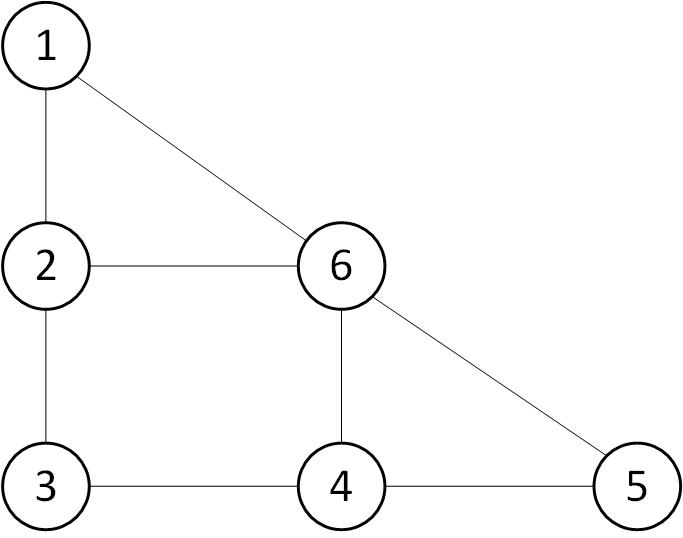
\includegraphics[width=0.3\textwidth]{fig1.jpg}
			\caption{车站之间公路连接情况}
		\end{center}\end{figure}

	\newpage
	\item 考察某一系统运作情况(如机器运转)。如果运作正常,则认为系统处于状态1;如果系统正在调整(例如机器维修,计算机杀毒等),则认为系统处于状态0。系统运作一段时间后,会遇到不能正常运作的情况,此时系统需要调整。调整后又恢复运作。假定系统从开始运作直到需要调整的运作时间是随机的,服从参数为\(\mu\)的指数分布,密度函数为\(\mu e^{-\mu t},t>0\)。而调整期也是随机的,服从参数为\(\lambda\)的指数分布,密度函数为\(\lambda e^{-\lambda t},t>0\)。假定运作周期是相互独立的,调整期也是相互独立的。如果令\(X(t)\)为系统在时刻\(t\)所处的状态,则由于在时刻\(t\)以后,系统所处的状态仅与在时刻\(t\)及其以后的剩余运作时间或剩余调整时间有关。利用指数分布的无记忆性知道,\(X(t)\)是时齐Markov链。利用Kolmogorov方程求出此Markov链的转移概率。
	\newpage
	\vspace{13em}
	\item 设今日有雨,则明日也有与的概率为0.7,今日无雨,明日有雨的概率为0.5。求星期一有雨,星期三也有雨的概率。
	\vspace{13em}
	\item 某人有\(r\)把伞用于上下班,如果一天的开始他在家(一天的结束他在办公室)中而且天下雨,只要有伞可取到,他将拿一把到办公室(家)中。如果天不下雨,那么他不带伞,假设每天的开始(结束)下雨的概率为\(p\),且与过去情况独立。
	\begin{enumerate}[\bfseries (1)]
		\item 定义一个有\(r+1\)个状态的Markov链并确定转移概率;
		\item 计算极限分布;
		\item 他被淋湿的平均次数所占比率是多少?(如果天下雨而全部伞在另一处,那么称他被淋湿)。
	\end{enumerate}
	\vspace{15em}
	\item 若\(f_{ii}<1,f_{jj}<1\),证明
	\begin{align*}
		 & \sum_{n=1}^{\infty}p_{ij}^{(n)}<+\infty                                            \\
		 & f_{ij}  =\frac{\sum_{n=1}^{\infty}p_{ij}^{(n)}}{1+\sum_{n=1}^{\infty}p_{jj}^{(n)}}
	\end{align*}
	\newpage

	\item 考虑有两个状态的连续时间Markov链,状态为0和1,链在离开0到达1之前在状态0停留的时间服从参数为\(\lambda\)的指数分布,相应地在1停留的时间是参数为\(\mu\)的指数变量。对此建立Markov微分方程,并求其解。
	\vspace{15em}
	\item 设有一质点在1,2,3上做随机跳跃,在时刻t它位于三点之一,且在\([t,t+h]\)内以概率\(\frac{1}{2}+o(h)\)分别可以跳到其他两个状态。试求状态概率满足的Kolmogorov方程。
\end{Exercises}
% LaTeX source for book ``代数学方法'' in Chinese
% Copyright 2018  李文威 (Wen-Wei Li).
% Permission is granted to copy, distribute and/or modify this
% document under the terms of the Creative Commons
% Attribution 4.0 International (CC BY 4.0)
% http://creativecommons.org/licenses/by/4.0/

% To be included
\chapter{鞅}

\begin{compactitem}
	\item 鞅的定义.
	\item 停时定理.
\end{compactitem}

\begin{definition}\label{def:martingale}\index{Yang@鞅 (Martingale)}
	如果\(\{\mathscr{F}_n,n\geqslant0\}\)是一个\(\mathscr{F}\)中的单调递增的子\(\sigma\)代数流。随机过程\(\{X_n,n\geqslant0\}\)称为关于\(\{\mathscr{F}_n,n\geqslant0\}\)的\emph{鞅},如果\(\{X_n\}\)是\(\{\mathscr{F}_n\}\)适应的,\(E(\lvert X_n\rvert)<\infty\),并且\(\forall n\geqslant0\),有
	\begin{align*}
		E(X_{n+1}|\mathscr{F}_n)=X_n
	\end{align*}
	适应列\(\{X_n,\mathscr{F}_n,n\geqslant0\}\)称为\emph{下鞅},如果\(\forall n \geqslant 0\),有
	\begin{align*}
		E(X_n^+)<\infty, \quad E(X_{n+1}|\mathscr{F}_n)\geqslant X_n
	\end{align*}
	\emph{上鞅}可类似定义。
\end{definition}

\(\sigma\)代数的概念是在提出概率空间时引入的,它是样本空间的某些子集组成的集合组。它表示这些子集可以被我们所度量,比如我们关心事件A发生的概率,我们也会去关系事件A不发生的概率,如果还有一个事件B,我们也会关心事件A和事件B同时发生的概率,等等。\(\sigma\)代数就是所有这些事件的组合的集合,这些事件的组合应当也是样本空间的子集。严格意义上,\(\sigma\)代数要满足补集运算和可数个并集运算的封闭性。

\(\sigma\)域流表示随时间演化的信息流,随机变量随着时间的增加产生更多的信息。\(\sigma\)域流需要满足信息随时间只增不减,以及\(\sigma\)代数的可测性。

不懂这些数学概念并不影响做题,因为通常情况下,\(\sigma\)代数流的要求都可以满足。但是需要知道,\textbf{鞅}是定义在一种规则(或信息)下的,在这个规则(或信息)下,随机过程的条件期望满足一些性质,离开了这个规则(或信息),鞅的定义便不存在。在鞅的定义中,条件期望所满足的条件,是用来描述这种规则(或信息)的。

\begin{theorem}[停时定理]\label{prop:Downtime}
	设\(\{X_n,n\geqslant 0\}\)是一个随机变量序列,称随机函数T是关于\(\{X_n,n\geqslant 0\}\)的\emph{停时},如果T在\(\mathbb{Z^+}\)中取值,且对每个\(n\geqslant 0,\{T=n\}\in \sigma(X_0,X_1,\cdots,X_n)\)。

	如果\(\{X_n,n\geqslant0\}\)是关于\(\{\mathscr{F}_n=\sigma(X_0,X_1,\cdots,X_n)\}\)的鞅,T是停时且满足
	\begin{enumerate}[\bfseries (1)]
		\item \(P\{T<\infty\}\),
		\item \(E(|M_T|)<+\infty\),
		\item \(\lim_{n\to \infty}E(|M_n|I_{\{T>n\}})=0\)
	\end{enumerate}
	则有
	\begin{align*}
		E(M_T)=E(M_0)
	\end{align*}
\end{theorem}

由定义可以发现\(\{T=n\}\)或\(\{T\neq n\}\)都应当由\(n\)时刻及其之前的信息完全确定,而不需要也无法借助将来的情况。借助赌博的例子,赌博者何时决定停止赌博只能以他已经赌过的结果为依据,而不能说,如果下一次要输,我现在就停止赌博,这时对停止时刻T的第一个要求:它必须是一个停时。

\begin{Exercises}
	\item 设\(Y_0,Y_1,Y_2,\cdots\)是一系列独立随机变量且\(E\lvert Y_n\rvert<+\infty,EY_n=0\)。令\(X_n=\sum_{i=0}^{n}Y_i,n=0,1,2,\cdots,\mathscr{F}_n=\sigma\{Y_i,i=0,1,2,\cdots,n\}\),则\(\{X_n,\mathscr{F}_n\}\)是一个鞅。
	\newpage
	\item 设\(Y_0,Y_1,Y_2,\ldots ,Y_n\)如上题假定,另外设\(EY^2_n=\sigma^2,n=1,2,\ldots,\)令\(Z_0,Z_n=\left(\sum_{i=1}^{n}Y_i\right)^2-n\sigma^2\),那么\(\{Z_n,\mathscr{F}_n\}\)是一个鞅。
	\vspace{30em}
	\item 令\(X_0,X_1,\cdots\)表示分支过程各代的个体数,\(X_0=1\),任意一个个体生育后代的分布有均值\(\mu\)。证明\(\{M_n=\mu^{-n}X_n\}\)是一个关于\(X_0,X_1,\cdots\)的鞅。
	\newpage
	\item 考虑一个在整数上的随机游动模型,设向右移动的概率\(p<\frac{1}{2}\),向左移动的概率为\(1-p,S_n\)表示时刻n所处的位置,假定\(S_0=a,0<a<N\)。
	\begin{enumerate}[\bfseries (1)]
		\item 证明:\(\{M_n=\left(\frac{1-p}{p}\right)^{S_n}\}\)是鞅;
		\item 令T表示随机游动第一次到达0或N的时刻,即
		      \begin{align*}
			      T=\min\{n:S_n=0orN\}
		      \end{align*}
		      利用鞅停时定理,求出\(P\{S_T=0\}\)。
	\end{enumerate}
\end{Exercises}
% LaTeX source for book ``代数学方法'' in Chinese
% Copyright 2018  李文威 (Wen-Wei Li).
% Permission is granted to copy, distribute and/or modify this
% document under the terms of the Creative Commons
% Attribution 4.0 International (CC BY 4.0)
% http://creativecommons.org/licenses/by/4.0/

% To be included
\chapter{Brown运动}

\begin{compactitem}
	\item Brown运动的定义.
	\item 正态增量、独立增量和路径连续性.
	\item Gauss过程的特点.
\end{compactitem}

\begin{definition}\label{def:BrownMotion}\index{brownyundong@Brown运动(Brown Motion)}
	随机过程\(\{X(t),t \geqslant 0 \}\)如果满足:
	\begin{enumerate}[\bfseries (1)]
		\item \(X(0)=0\);
		\item \(\{X(t),t\geqslant 0\}\);
		\item 对每个\(t>0,X(t)\)服从正态分布\(N(0,\sigma^2t)\)。
	\end{enumerate}
	则称\(X(t),t \geqslant 0\)为\textbf{Brown运动},也称为\emph{Wiener过程},记为\(\{B(t),t\geqslant0\}\)或\(\{W(t),t\geqslant0\}\)。
\end{definition}

Brown运动\(\{B(t),t,\geqslant 0\}\)具有以下性质:
\begin{itemize}[\bfseries (1)]
	\item (正态增量过程)\(\forall 0\leqslant s <t,B(t)-B(s)\sim N(0,t-s)\),即\(\{B(t)-B(s)\}\)服从均值为0,方差为\(t-s\)的正态分布。当\(s=0\)时,\(B(t)-B(0)\sim N(0,t)\)。
	\item (独立增量)\(\forall 0\leqslant s <t,B(t)-B(s)\)独立于过程过去的状态\(B(u),0\leqslant u<s\)。
	\item (路径的连续性)\(\{B(t)(t\geqslant0)\}\)是t的连续函数。
\end{itemize}

不失一般性,假设\(B(0)=0\)。

\begin{definition}\label{def:QuadraticVariation}\index{ercibiancha@二次变差(Quadratic Variation)}
	Brown运动的\emph{二次变差}\([B,B](t)\)定义为党\(\{t_i^n\}_{i=0}^n\)取遍\([0,t]\)的分割,且其模
	\(\delta_n=\underset{0\leqslant i\leqslant n-1}{\max}\{t_{i+1}^{n}-t_{i}^n\}\to 0\)时,依概率收敛意义下的极限
	\begin{align*}
		[B,B](t)=[B,B]([0,t])=\underset{\delta_n \to 0}{\lim}\sum_{i=0}^{n-1}
		\lvert B(t_{i+1}^n)-B(t_i^n) \rvert^2
	\end{align*}
\end{definition}

类似的,一次变差的定义为\(\underset{\delta_n \to 0}{\lim}\sum_{i=0}^{n-1}\lvert B(t_{i+1}^n)-B(t_i^n) \rvert\)。

从时刻0到时刻t对Brown运动的一次观察称为Brown运动在区间[0,T]上的一个路径或一个实现。Brown运动的几乎所有样本路径
\(B(t)(0\leqslant t\leqslant T)\)都具有下述性质:
\begin{enumerate}[\bfseries (1)]
	\item 是\(t\)的连续函数;
	\item 在任意区间(无论区间多么小)上都不是单调的;
	\item 在任意点都不是可微的;
	\item 在任意区间(无论区间多么小)上都是无限变差的(一次变差);
	\item 对任意\(t\),在区间\([0,t]\)上的二次变差等于\(t\)。
\end{enumerate}

对任意过程,如果一次变差是有限值,那么二次变差一定是0。对于Brown运动,二次变差是有限值,一次变差是无穷大。

\begin{theorem}[多元正态分布的性质]\label{prop:MultiNormDist}
	设\(X\sim \mathcal{N}(\mu_1,\sigma^2_1),Y\sim \mathcal{N}(\mu_2,\sigma_2^2)\)是相互独立的,
	则\((X+Y)\sim \mathcal{N}(\boldsymbol{\mu},\boldsymbol{\Sigma})\)。其中均值
	\(\boldsymbol{\mu }=(\mu_1,\mu_1+mu_2)'\),协方差矩阵
	\(\boldsymbol{\Sigma}=\begin{pmatrix}
		\sigma_1^2 & \sigma_1^2            \\
		\sigma_1^2 & \sigma_1^2+\sigma_2^2
	\end{pmatrix}\)。
\end{theorem}

\begin{theorem}[Brown运动是Gauss过程]\label{prop:GaussProcess}
	Brown运动是均值函数为\(m(t)=0\)、协方差函数为\(\gamma (s,t)=\min\{t,s\}\)的Gauss过程。
\end{theorem}

\newpage
\begin{Exercises}
	\item 设\(\{B(t),t\geqslant0\}\)是标准Brown运动,计算\(P\{B(2)\leqslant0\}\)和\(P\{B(t),\leqslant0,t=0,1,2\}\)。
	\vspace{30em}
	\item 设\(\{B(t)\}\)是Brown运动,求\(B(1)+B(2)+B(3)+B(4)\)的分布。
	\newpage
	\item 求\(B(\frac{1}{4})+B(\frac{1}{2})+B(\frac{3}{4})+B(1)\)的分布.
	\vspace{30em}
	\item 求概率\(P\{\int_{0}^{1} B(t)dt>\frac{2}{\sqrt{3}}\}\)
\end{Exercises}
% LaTeX source for book ``代数学方法'' in Chinese
% Copyright 2018  李文威 (Wen-Wei Li).
% Permission is granted to copy, distribute and/or modify this
% document under the terms of the Creative Commons
% Attribution 4.0 International (CC BY 4.0)
% http://creativecommons.org/licenses/by/4.0/

% To be included
\chapter{随机积分}

\begin{compactitem}
	\item It\(\hat{o}\)积分.
	\item It\(\hat{o}\)公式和It\(\hat{o}\)引理.
	\item 简单微分方程的解法.
\end{compactitem}

\begin{definition}\label{def:ItoInt}\index{yitengjifen@Ito积分(Ito Integrate)}
	设\(f\in V(0,T)\),则\(f\)的\emph{It\(\hat{o}\)积分}定义为:
	\begin{align*}
		\int_0^T f(t,\omega)dB_t(w)=\underset{n\to \infty}{\lim}
		\int_0^T \phi_n(t,\omega)dB_t(\omega)
	\end{align*}
	这里\(\{\phi _n\}\)是初等随机过程的序列,使得当\(n\to \infty\)时,有
	\begin{align*}
		E\left\{ \int_0^T[f(t,\omega)-\phi_n(t,\omega)]^2dt\right\}\to 0
	\end{align*}
\end{definition}

\begin{definition}\label{def:ItoIntpro}\index{yitengjifenguocheng@Ito积分过程(Ito Integrate process)}
	假设对任意实数\(T>0,X\in V^*\),那么\(\forall t\leqslant T\),积分\(\int_0^t X(s)dB(s)\)是适定的。
	因为对任意固定的\(t,\int_0^t X(s)dB(s)\)是一个随机变量,所以作为上限t的函数,它定义了一个随机过程
	\(\{Y(t)\}\),称为\emph{It\(\hat{o}\)积分过程},其中
	\begin{align*}
		Y(t)=\int_0^t X(s)dB(s)
	\end{align*}
	可以证明,It\(\hat{o}\)积分过程存在连续的样本路径。
\end{definition}

\begin{theorem}[It\(\hat{o}\)公式]\label{prop:ItoFormula}
	设g是有界连续函数,\(\{t_i^n\}\)是\([0,t]\)的分割,则\(\forall\theta_i^n \in (B(t_i^n),B(t^n_{i+1}))\),
	依概率收敛意义下的极限
	\begin{align*}
		\underset{\delta_n \to 0}{\lim}\sum_{i=0}^{n-1}g(\theta_i^n)[B(t_{i+1}^n)-B(t_i^n)]^2=\int_0^tg[B(s)]ds
	\end{align*}
\end{theorem}

\begin{theorem}[Brown运动的It\(\hat{o}\)公式]\label{prop:ItoFormulaofBrownProcess}
	如果\(f\)是二次连续可微函数,则对任意\(t\),有
	\begin{align*}
		f[B(t)]=f(0)+\int_0^tf'[B(s)]dB(s)+\frac{1}{2}\int_0^tf''[B(s)]ds
	\end{align*}
\end{theorem}

\begin{definition}[It\(\hat{o}\)过程(积分形式)]\label{prop:ItoProcess(Int)}
	如果过程\(\{Y(t),0\leqslant t\leqslant T\}\)可以表示为:
	\begin{align*}
		Y(t)=Y(0)+\int_0^t\mu(s)ds+\int_0^t\sigma(s)dB(s),\quad 0\leqslant t\leqslant T
	\end{align*}
	其中过程\(\{\mu(t)\}\)和\(\{\sigma(t)\}\)满足
	\begin{enumerate}[\bfseries (1)]
		\item \(\mu(t)\)是适应的并且\(\int_0^T\lvert \mu(t)\rvert dt<\infty,a.s.\);
		\item \(\sigma(t)\in V^*\).
	\end{enumerate}
	则称\(\{Y(t)\}\)为\emph{It\(\hat{o}\)过程}.
\end{definition}

有时也将It\(\hat{o}\)过程记为微分形式:
\begin{align*}
	dY(t)=\mu(t)dt+\sigma(t)dB(t),\quad 0\leqslant y\leqslant T
\end{align*}
式中,函数\(\mu(t)\)称为漂移系数,\(\sigma(t)\)称为扩散系数。

\begin{theorem}[It\(\hat{o}\)过程的It\(\hat{o}\)公式]\label{prop:ItoFormulaofItoProcess}
	设\(\{X(t)\}\)是由
	\begin{align*}
		dX(t)=\mu(t)dt+\sigma(t)dB(t)
	\end{align*}
	给出的It\(\hat{o}\)过程,\(g(t,x)\)是\([0,\infty) \times  \mathbb{R} \)
	上的二次连续可微函数,则
	\begin{align*}
		\{Y(t)=g[t,X(t)]\}
	\end{align*}
	仍为It\(\hat{o}\)过程,并且
	\begin{align*}
		dY(t)=\frac{\partial g}{\partial t}[t,X(t)]dt+\frac{\partial g}{\partial x}[t,X(t)]dX(t)
		+\frac{1}{2}\frac{\partial^2 g}{\partial x^2}[t,X(t)][dX(t)]^2
	\end{align*}
	可以简化为:
	\begin{align*}
		dY(t)dt=\{g'[X(t)]\mu(t)+\frac{1}{2}g''[X(t)]\sigma^2(t)\}dt+g'[X(t)]\sigma(t)dB(t)
	\end{align*}
\end{theorem}

\begin{Exercises}
	\item 求\(d(e^{B(t)})\)
	\vspace{15em}
	\item 求解Ornstein-Uhlenbeck方程
	\begin{align*}
		dX_t=-\mu X_tdt+\sigma dB_t
	\end{align*}。
	其中\(\mu,\sigma\)为常数。
	\newpage
	\item 考虑群体增长模型
	\begin{align*}
		\frac{dN_t}{dt}=a_tN_t
	\end{align*}
	其中\(N_0\)已知,\(a_t=r_t+\alpha B_t\),\(r_t\)为增长率,假设为常数\(r\),\(\alpha\)为常数,\(B_t\)为Brown运动。可以将其化为随机微分方程的形式
	\begin{align*}
		dN_t=rN_tdt+\alpha N_tdB_t
	\end{align*}
	这种类型的方程被称为集合随机微分方程,试求解它。
	\newpage
	\item 设\(X(t)\)具有随机微分形式
	\begin{align*}
		dX(t)=(bX(t)+c)dt+2\sqrt{X(t)}dB(t)
	\end{align*}
	并假定\(X(t)\geqslant0\),试找出过程\(\{Y(t)=\sqrt{X(t)}\}\)的随机微分形式。
	\newpage
	\item 利用It\(\hat{o}\)公式证明
	\begin{align*}
		\int_{0}^{t}B^2(s)ds=\frac{1}{3}B^3(t)-\int_{0}^{t}B(s)ds
	\end{align*}
	\vspace{15em}
	\item 设\(\{X(t),Y(t)\}\)是It\(\hat{o}\)过程,试证
	\begin{align*}
		d(X(t)Y(t))=X(t)dY(t)+Y(t)dX(t)+dX(t)\cdot dY(t)
	\end{align*}
	由此导出下面的分部积分公式
	\begin{align*}
		\int_{0}^{t}X(s)dY(s)=X(t)Y(t)-X(0)Y(0)-\int_{0}^{t}Y(s)dX(s)-\int_{0}^{t}dX(s)\cdot dY(s)
	\end{align*}
\end{Exercises}
% LaTeX source for book ``代数学方法'' in Chinese
% Copyright 2018  李文威 (Wen-Wei Li).
% Permission is granted to copy, distribute and/or modify this
% document under the terms of the Creative Commons
% Attribution 4.0 International (CC BY 4.0)
% http://creativecommons.org/licenses/by/4.0/

% To be included
\chapter{习题答案}

\section{随机变量}

\begin{enumerate}
	\item 设\(\{X(t),t\in T\}\)是一、二阶矩存在的随机过程。试证明它是宽平稳的当且仅当\(E(X(s))\)与\(E(X(s)X(s+t))\)都不依赖于\(s\)。

	      \textbf{充分性:}\(\gamma(t,s)=E(X(s)X(t+s))-E(X(s))E(X(s+t))\),由于\(\forall t,s\in T,E(X(s))\)和\(E(X(s+t))\)均不依赖于\(s\),所以均值函数为定值,记为\(\mu_X\),则\(\gamma(t,s)=E(X(s)X(t+s))-\mu_X^2\)仅与时间差\(t=t+s-s\)有关,所以\(\{X(t),t\in T\}\)为宽平稳过程。

	      \textbf{必要性:}\(\gamma(t,s)=E(X(s)X(t+s))-E(X(s))E(X(s+t))\)仅与时间差\(t+s-s=t\)有关。由宽平稳过程可知,均值函数为定值,记为\(\mu_X\),\(E(X(s+t))=E(X(s))=\mu_X\),即\(E(X(s))\)不依赖于\(s\)。\(E(X(s)X(t+s))=E(X(s))E(X(s+t))+\gamma(t,s)=\mu_X^2+\gamma(t,s)\)仅与时间差\(t\)有关,不依赖于\(s\)。

	\item 若\(Z_0,Z_1,\cdots\)为独立同分布随机变量,定义\(X_n=Z_0+Z_1+\cdots+Z_n\),则\({X_n,n\geqslant0}\)是独立增量过程。

	      由于\(Z_0,Z_1,\cdots\)独立同分布,所以\(\{X_n-X_{n-1}=Z_n,n=1,2,\cdots \}\)相互独立,即\(\{X_n,n\geqslant0\}\)为独立增量过程。

	\item 设\(Z_1,Z_2\)是独立同分布的随机变量,服从均值为0,方差为\(\sigma^2\)的正态分布,\(\lambda\)为实数。求过程\(\{X(t),t\in T\}\),其中\(X(t)=Z_1\cos \lambda t+Z_2 \sin \lambda t\)的均值函数和方差函数。它是宽平稳的吗?

	      由于\(E(Z_1)=E(Z_2)=0,E(X(t))=E(Z_1)\cos\lambda t+E(Z_2)\sin \lambda t=0\)。

	      由于\(Var(Z_1)=Var(Z_2)=\sigma^2\),
	      \begin{align*}
		      Var(X(t)) & =Var(Z_1)\cos^2\lambda t+Var(Z_2)\sin^2 \lambda t \\
		                & =\sigma^2(\cos^2\lambda t+\sin^2 \lambda t)       \\
		                & =\sigma^2
	      \end{align*}

	      由于\(Z_1,Z_2\)是独立的,所以\(E(Z_1Z_2)=E(Z_1)E(Z_2)=0\)。
	      \begin{align*}
		      \gamma(t,s)
		      =  E      & (X(t)X(s))-E(X(t))E(X(s))                                                           \\
		      =  E      & \left[(Z_1\cos\lambda t+Z_2\sin\lambda t)(Z_1\cos\lambda s+Z_2\sin\lambda s)\right] \\
		      =  E      & [Z_1^2\cos \lambda t \cos \lambda s+Z_2^2\sin \lambda t \sin \lambda s              \\
		                & +Z_1Z_2(\cos \lambda t \sin \lambda s+\cos \lambda s \sin \lambda t)]               \\
		      =  E      & (Z_1^2)\cos \lambda t \cos \lambda s +E(Z_2^2)\sin \lambda t \sin \lambda s         \\
		                & +E(Z_1Z_2)(\cos \lambda t \sin \lambda s+\cos \lambda s \sin \lambda t)             \\
		      =\sigma^2 & (\cos \lambda t \cos \lambda s+\sin \lambda t \sin \lambda s)                       \\
		      =\sigma^2 & \cos\lambda(t-s)
	      \end{align*}
	      仅与时间差\(t-s\)有关,并且\(E(X(t))=0\)为定值,\(\{X(t)\}\)的一二阶矩已知,所以\(\{X(t),t\in T\}\)是宽平稳过程。
\end{enumerate}
\section{Poisson过程}
\textbf{Poisson过程定义1}:

计数过程\(N(t),t\geqslant 0\)则称为参数为\(\lambda (\lambda >0 )\)的\emph{Possion过程},如果
\begin{enumerate}[\bfseries (1)]
	\item \(N(0)=0\)
	\item 过程具有独立增量
	\item 在任意长度为t的时间区间中事件发生次数服从均值为\(\lambda t\)的Poission分布,即对一切\(s\geqslant 0,t>0\),有\begin{align*}P\{N(t+s)-N(s)=n\}=e^{-\lambda t}\frac{(\lambda t)^n}{n!},\quad n=0,1,2,\cdots\end{align*}
\end{enumerate}

\textbf{Poisson过程定义2}:

设\(N(t),t\geqslant 0\)是一个计数过程,它满足
\begin{enumerate}[\bfseries \((1)^{\prime}\)]
	\item \{N(0)=0\};
	\item 过程具有平稳独立增量
	\item 存在\(\lambda>0\),当\(h\downarrow 0\)时,有
	      \begin{align*}
		      P\{N(t+h)-N(t)=1\}=\lambda h+o(h)
	      \end{align*}
	\item 当\(h\downarrow 0\)时,有
	      \begin{align*}
		      P\{N(t+h)-N(t)\geqslant 2\}=o(h)
	      \end{align*}
\end{enumerate}
则\(\{N(t),t\geqslant 0\}\)是参数为\(\lambda\)的\emph{Possion过程}。

\begin{enumerate}
	\item 证明以上两种Poisson过程的定义等价。
	      \begin{enumerate}[\bfseries 1)]
		      \item 首先证明定义1可以推得定义2:
		            \begin{itemize}

			            \item \((1){\prime}\)显然满足。

			            \item 根据(3)中概率分布\(P\{N(t+s)-N(t)=n\}=e^{-\lambda t}\frac{(\lambda t)^n}{n!}\)与\(s\)无关,所以\(\{N(t),t\geqslant 0\}\)是平稳增量过程,结合(2)可知\((2)^{\prime}\)。

			            \item 当\(h\to 0^+\)时,\(P\{N(t+h)-N(t)=1\}=e^{-\lambda h}\lambda h=(1-\lambda h+o(h))\lambda h=\lambda h+o(h)\)。

			            \item 当\(h\to 0^+\)时,\(P\{N(t+h)-N(t)\geqslant 2\}=\sum_{n=2}^{+\infty}e^{-\lambda h}\frac{(\lambda h)^n}{n!}=(1-\lambda h+o(h))o(h)=o(h)\)。

		            \end{itemize}
		      \item 其次证明定义2可以推得定义1:
		            \begin{itemize}

			            \item (1),(2)显然满足。

			            \item 首先求\(P\{N(t)\}=0\):
			                  \begin{align*}
				                  P  & \{N(t+h)=0\}                                       \\
				                  =P & \{N(t)=0,N(t+h)-N(t)=0\}                           \\
				                  =P & \{N(t)=0\}P\{N(t+h)-N(t)=0\}                       \\
				                  =P & \{N(t)=0\}                                         \\
				                     & (1-P\{N(t+h)-N(t)=1\}-P\{N(t+h)-N(t)\geqslant 2\}) \\
				                  =P & \{N(t)=0\}(1-\lambda t +o(h))
			                  \end{align*}
			                  整理得到
			                  \begin{align*}
				                  \frac{P\{N(t+h)=0\}-P\{N(t)=0\}}{h}=-\lambda P\{N(t)=0\} +o(h)
			                  \end{align*}
			                  令\(h\to 0^+\),
			                  \begin{align*}
				                  P^{\prime}\{N(t)=0\}=-\lambda P\{N(t)=0\}
			                  \end{align*}
			                  解得\(P\{N(t)=0\}=C e^{-\lambda t}\),由\(P\{N(0)=0\}\)得到\(P\{N(t)=0\}=e^{-\lambda t}\)。

			            \item 然后利用\((3)^{\prime}\)和\((4)^{\prime}\)得到\(P\{N(t)=n\}\)和\(P\{N(t)=n-1\}\)的递推关系(微分方程)。
			                  \begin{align*}
				                  P  & \{N(t+h)=n\}                                        \\
				                  =P & \{N(t)=n-1,N(t+h)-N(t)=1\}                          \\
				                     & +P\{N(t)=n,N(t+h)-N(t)=0\}+o(h)                     \\
				                  =P & \{N(t)=n-1\}(\lambda h+o(h))                        \\
				                     & +P\{N(t)=n\}(1-\lambda h+o(h))+o(h)                 \\
				                  =P & \{N(t)=n-1\}\lambda h+P\{N(t)=n\}(1-\lambda h)+o(h) \\
			                  \end{align*}
			                  整理得到
			                  \begin{align*}
				                  \frac{P\{N(t+h)=n\}-P\{N(t)=n\}}{h}=-\lambda (P\{N(t)=n\}-P\{N(t)=n-1\})
			                  \end{align*}
			                  令\(h\to 0^+\)
			                  \begin{align*}
				                  \frac{d}{dt}P\{N(t)=n\}=-\lambda P\{N(t)=n\}+\lambda P\{N(t)=n\}
			                  \end{align*}
			                  等价于
			                  \begin{align*}
				                  \frac{d}{dt}\{e^{\lambda t}P\{N(t)=n\}=e^{\lambda t}P\{N(t)=n-1\}\}
			                  \end{align*}

			            \item 结合\((2)^{\prime}\)平稳独立增量的条件,利用数学归纳法得到(3):

			                  当\(n=0\)时,有
			                  \begin{align*}
				                   & \left\{
				                  \begin{matrix}
					                  \frac{d}{dt}\{e^{\lambda t} P\{N(t)=1\}\}=e^{\lambda t}P\{N(t)=0\}
					                  =\lambda e^{\lambda t}e^{-\lambda t}=\lambda \\
					                  P\{N(0)=1\}=0
				                  \end{matrix}
				                  \right.                                             \\
				                   & \Rightarrow P\{N(t)=1\}=\lambda t e^{-\lambda t}
			                  \end{align*}
			                  假设\(P\{N(t)=n-1\}=e^{-\lambda t}\frac{(\lambda t)^n}{(n-1)!}\)。

			                  \begin{align*}
				                  \frac{d}{dt}\{e^{-\lambda t}P\{N(t)=n\}\}
				                   & =\lambda e^{\lambda t}P\{N(t)=n-1\}                              \\
				                   & =\lambda e^{\lambda t}e^{-\lambda t}\frac{(\lambda t)^n}{(n-1)!} \\
				                   & =\lambda \frac{(\lambda t)^{n-1}}{(n-1)!}
			                  \end{align*}
			                  由\(e^{\lambda t}P\{N(t)=n\}|_{t=0}=0\),得到\(e^{\lambda t}P\{N(t)=n\}=\frac{(\lambda t)^n}{n!}\),\(P\{N(t)=n\}=e^{-\lambda t}\frac{(\lambda t)^n}{n!}\),所以\(P\{N(t)=n\}=P\{N(t+0)-N(t)=n\}=e^{-\lambda t}\frac{(\lambda t)^n}{n!}\)
		            \end{itemize}

	      \end{enumerate}
	\item 设\(\{N(t),t\geqslant0\}\)是参数\(\lambda=3\)的Poisson过程。试求
	      \begin{itemize}[\bfseries 1)]
		      \item \(P\{N(1)\leqslant3\}\);
		      \item \(P\{N(1)=1,N(3)=2\}\);
		      \item \(P\{N(1)\geqslant2|N(1)\geqslant1\}\)。
	      \end{itemize}

	      \begin{enumerate}[\bfseries 1)]
		      \item \begin{align*}
			            P\{N(1)\leqslant 3\}
			             & =P\{N(1)=0\}+P\{N(1)=1\}+P\{N(1)=2\}+P\{N(1)=3\}   \\
			             & =e^{-\lambda}(1+\lambda+\lambda^2/2!+\lambda^3/3!) \\
			             & =13e^{-3}
		            \end{align*}
		      \item \begin{align*}
			            P\{N(t)=1,N(3)=2\}
			             & =P\{N(1)=1,N(3)-N(1)=1\}                   \\
			             & =P\{N(1)=1\}P\{N(3)-N(1)=1\}               \\
			             & =P\{N(1)=1\}P\{N(2)=1\}                    \\
			             & =\lambda e^{-\lambda}e^{-2\lambda}2\lambda \\
			             & =2\lambda^2e^{-3\lambda}                   \\
			             & =18e^{-9}
		            \end{align*}
		      \item \begin{align*}
			            P\{N(1)\geqslant2|N(1)\geqslant1\}
			             & =\frac{P\{N(1)\geqslant2,N(1)\geqslant1\}}{P\{N(1)\geqslant1\}} \\
			             & =\frac{P\{N(1)\geqslant2\}}{P\{N(1)\geqslant1\}}                \\
			             & =\frac{1-P\{N(1)\leqslant1\}}{1-P\{N(1)=0\}}                    \\
			             & =\frac{1-e^{-\lambda}-\lambda e^{-\lambda}}{1-e^{-\lambda}}     \\
			             & =\frac{1-4e^{-3}}{1-e^{-3}}
		            \end{align*}
	      \end{enumerate}
	\item 对于Poisson过程\(\{N(t)\}\),证明当\(s<t\)时,
	      \begin{align*}
		      P\{N(s)=k|N(t)=n\}={n\choose k}\left(\frac{s}{t}\right)^k\left(1-\frac{s}{t}\right)^{n-k},\quad k=0,1,2,\ldots,n
	      \end{align*}

	      \begin{align*}
		      P\{N(s)=k|N(t)=n\}
		       & =\frac{P\{N(s)=k,N(t)=n\}}{P\{N(t)=n\}}                                                                \\
		       & =\frac{P\{N(s)=k,N(t)-N(s)=n-k\}}{P\{N(t)=n\}}                                                         \\
		       & =\frac{P\{N(s)=k\}P\{N(t)-N(s)=n-k\}}{P\{N(t)=n\}}                                                     \\
		       & =\frac{P\{N(s)=k\}P\{N(t-s)=n-k\}}{P\{N(t)=n\}}                                                        \\
		       & =\frac{e^{-\lambda s}\frac{(\lambda s)^k}{k!}e^{-\lambda (t-s)}\frac{(\lambda (t-s))^{n-k}}{(n-k)!}}
		      {e^{-\lambda t}\frac{(\lambda t)^n}{n!}}                                                                  \\
		       & =\frac{e^{-\lambda s}e^{-\lambda (t-s)}}{e^{-\lambda t}}\cdot \frac{\lambda^k\lambda^{n-k}}{\lambda^n}
		      \cdot \frac{s^k(t-s)^{n-k}}{t^n}\cdot \frac{n!}{k!(n-k)!}                                                 \\
		       & ={n\choose k}\bigg(1-\frac{s}{t} \bigg)^{n-k}\bigg(\frac{s}{t}\bigg)^k
	      \end{align*}

	\item 设\(\{N_1(t)\}\)和\(\{N_2(t)\}\)分别是参数为\(\lambda_1,\lambda_2\)的Poisson过程,令\(X(t)=N_1(t)-N_2(t)\),问\(\{X(t)\}\)是否为Poisson过程,为什么?

	      由于\(N_1(t)\sim Poisson(\lambda_1t),N_2(t)\sim Poissin(\lambda_2t)\)。

	      \textbf{方法一:}

	      \begin{align*}
		      E[X(t)]   & =E[N_1(t)]-E[N_2(t)]=(\lambda_1-\lambda_2)t     \\
		      Var[X(t)] & =Var[N_1(t)]+Var[N_2(t)]=(\lambda_1+\lambda_2)t
	      \end{align*}
	      由于\(E[X(t)]\neq Var[X(t)]\),所以\(X(t)\)不服从Poisson分布,\(\{X(t)\}\)不是Poisson过程。

	      \textbf{方法二:}

	      由\(N_1(t)\sim Poisson(\lambda_1t)\)知\(P\{N_1(t)=n\}=e^{-\lambda_1t}\frac{(\lambda_1t)^n}{n!}\),
	      对应的特征函数为
	      \begin{align*}
		      \psi_{N_1}(r)
		       & =\sum_{n=0}^{\infty}e^{irn}P\{N_1(t)=n\}                                \\
		       & =\sum_{n=0}^{\infty}e^{irn}e^{(-\lambda_1 t)}\frac{(\lambda_1 t)^n}{n!} \\
		       & =\sum_{n=0}^{\infty}e^{(-\lambda_1 t)}\frac{(e^{ir}\lambda_1 t)^n}{n!}  \\
		       & =e^{\lambda_1 t e^{ir}}e^{-\lambda_1 t}                                 \\
		       & =e^{(e^{ir}-1)\lambda_1 t}
	      \end{align*}
	      同理可以得到\(\psi_{N_2}(r)=e^{(e^{ir}-1)\lambda_2 t}\),\(\psi_{-N_2}(r)=\psi_{N_2}(-r)=e^{(e^{-ir}-1)\lambda_2 t}\),所以
	      \begin{align*}
		      \psi_{X}(r)
		       & =\psi_{N_1}(r)\psi_{-N_2}(r)                                                   \\
		       & =e^{(e^{ir}-1)\lambda_1 t}e^{(e^{-ir}-1)\lambda_2 t}                           \\
		       & =\exp\left[e^{ir}\lambda_1 t+e^{-ir} \lambda_2 t-(\lambda_1+\lambda_2)t\right]
	      \end{align*}
	      由特征函数的唯一性定理知\(X(t)\)不服从Poisson分布,\(\{X(t)\}\)不是Poisson过程。
\end{enumerate}

\section{Markov链}

\begin{enumerate}
	\item 有6个车站,车站中间的公路连接情况如图\ref{fig:road2}所示。汽车每天可以从一个站驶向与之直接相邻的车站,并在夜晚达到车站留宿,次日凌晨重复相同的活动。设每天凌晨汽车开往临近的任何车站都是等可能的,试说明很长时间后,各车站每晚留宿的汽车比例趋于稳定。求出这个比例以便正确地设置各站的服务规模。
	      \begin{figure}[h!]\label{fig:road2}
		      \begin{center}
			      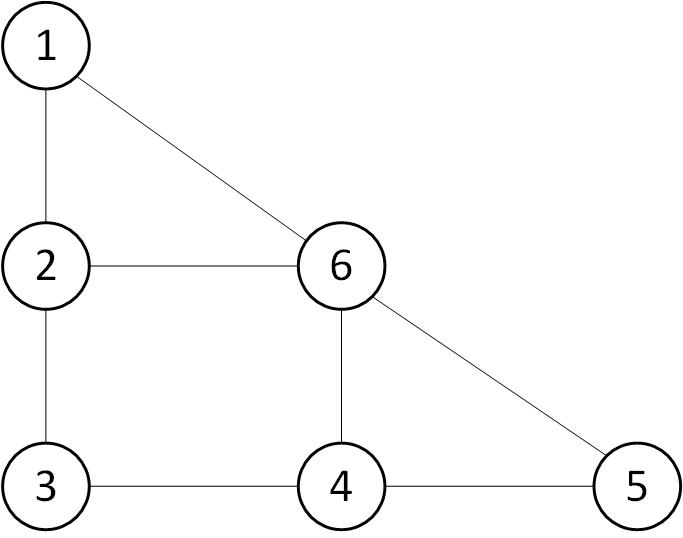
\includegraphics[width=0.3\textwidth]{fig1.jpg}
			      \caption{车站之间公路连接情况}
		      \end{center}\end{figure}

	      记\(X_n\)为第\(n\)天某辆汽车留宿的车站号。由于每天凌晨汽车开往临近的任何车站都是等可能的,所以\(\{X_n,n=0,1,2,\ldots\}\)是一个时齐Markov链。记\(p_{ij}^{(n)}\)为第\(n\)天汽车从\(i\)站开往\(j\)站的概率,则状态转移矩阵可以写为
	      \begin{align*}
		      \mathbf{P}=\begin{pmatrix}
			                 0   & 1/2 & 0   & 0   & 0   & 1/2 \\
			                 1/3 & 0   & 1/3 & 0   & 0   & 1/3 \\
			                 0   & 1/2 & 0   & 1/3 & 0   & 0   \\
			                 0   & 0   & 1/3 & 0   & 1/3 & 1/3 \\
			                 0   & 0   & 0   & 1/2 & 0   & 1/2 \\
			                 1/4 & 1/4 & 0   & 1/4 & 1/4 & 0
		                 \end{pmatrix}
	      \end{align*}
	      记\(\boldsymbol{\pi}=\begin{pmatrix}\pi_1&\pi_2&\pi_3&\pi_4&\pi_5&\pi_6\end{pmatrix}\)为平稳概率分布。

	      \textbf{方法一:} 解方程\(\boldsymbol{\pi}\mathbf{P}=\boldsymbol{\pi}\):

	      \(\boldsymbol{\pi}\mathbf{P}=\boldsymbol{\pi}\Rightarrow \mathbf{P}^T\boldsymbol{\pi}^T=\boldsymbol{\pi}^T\Rightarrow (\mathbf{P}^T-\mathbf{I})\boldsymbol{\pi}^T=\mathbf{0}\)。

	      其中\((\mathbf{P}^T-\mathbf{I})\)的前五行记为\(\mathbf{A}\),可以写为
	      \begin{align*}
		      \mathbf{A}=
		      \begin{pmatrix}
			      -1  & 1/3 & 0   & 0   & 0   & 1/4 \\
			      1/2 & -1  & 1/2 & 0   & 0   & 1/4 \\
			      0   & 1/3 & -1  & 1/3 & 0   & 0   \\
			      0   & 0   & 1/2 & -1  & 1/2 & 1/4 \\
			      0   & 0   & 0   & 1/3 & -1  & 1/4
		      \end{pmatrix}
	      \end{align*}
	      对\(\mathbf{A}\)进行初等行变换:
	      \begin{align*}
		       & \mathbf{A}=
		      \begin{pmatrix}
			      -1  & 1/3 & 0   & 0   & 0   & 1/4 \\
			      1/2 & -1  & 1/2 & 0   & 0   & 1/4 \\
			      0   & 1/3 & -1  & 1/3 & 0   & 0   \\
			      0   & 0   & 1/2 & -1  & 1/2 & 1/4 \\
			      0   & 0   & 0   & 1/3 & -1  & 1/4
		      \end{pmatrix}                                  \\
		       & \overset{1/2*r_1+r_2\rightarrow r_2}{\longrightarrow }
		      \begin{pmatrix}
			      -1 & 1/3  & 0      & 0    & 0 & 1/4 \\
			      0  & -5/3 & 1      & 0    & 0 & 3/4 \\
			      0  & 1/3  & -1     & 1 /3 & 0 & 0   \\
			         &      & \cdots &      &         \\
			         &      & \cdots &      &
		      \end{pmatrix}                                \\
		       & \overset{1/5*r_2+r_3\rightarrow r_3}{\longrightarrow }
		      \begin{pmatrix}
			      -1 & 1/3  & 0      & 0   & 0   & 1/4  \\
			      0  & -5/3 & 1      & 0   & 0   & 3/4  \\
			      0  & 0    & -4/5   & 1/3 & 0   & 3/20 \\
			      0  & 0    & 1/2    & -1  & 1/2 & 1/4  \\
			         &      & \cdots &     &
		      \end{pmatrix}                              \\
		       & \overset{8*(5/8*r_3+r_4)\rightarrow r_4}{\longrightarrow }
		      \begin{pmatrix}
			      -1 & 1/3  & 0    & 0     & 0  & 1/4  \\
			      0  & -5/3 & 1    & 0     & 0  & 3/4  \\
			      0  & 0    & -4/5 & 1/3   & 0  & 3/20 \\
			      0  & 0    & 0    & -19/3 & 4  & 11/4 \\
			      0  & 0    & 0    & 1/3   & -1 & 1/4
		      \end{pmatrix}                               \\
		       & \overset{19/15*(1/19*r_4+r_5)\rightarrow r_5}{\longrightarrow }
		      \begin{pmatrix}
			      -1 & 1/3  & 0    & 0     & 0  & 1/4  \\
			      0  & -5/3 & 1    & 0     & 0  & 3/4  \\
			      0  & 0    & -4/5 & 1/3   & 0  & 3/20 \\
			      0  & 0    & 0    & -19/3 & 4  & 11/4 \\
			      0  & 0    & 0    & 0     & -1 & 1/2
		      \end{pmatrix}                               \\
		       & \overset{1/19*(4*r_4+r_3)\rightarrow r_3}{\longrightarrow }
		      \begin{pmatrix}
			      -1 & 1/3  & 0    & 0    & 0  & 1/4  \\
			      0  & -5/3 & 1    & 0    & 0  & 3/4  \\
			      0  & 0    & -4/5 & 1/3  & 0  & 3/20 \\
			      0  & 0    & 0    & -1/3 & 0  & 1/4  \\
			      0  & 0    & 0    & 0    & -1 & 1/2
		      \end{pmatrix}                                \\
		       & \overset{1/2*r_5+r_4\rightarrow r_4}{\longrightarrow }
		      \begin{pmatrix}
			        &   & \cdots &      &           \\
			        &   & \cdots &      &           \\
			      0 & 0 & -4/5   & 1/3  & 0  & 3/20 \\
			      0 & 0 & 0      & -1/3 & 0  & 1/4  \\
			      0 & 0 & 0      & 0    & -1 & 1/2
		      \end{pmatrix}                                  \\
		       & \overset{5/2*(r_4+r_3)\rightarrow r_3}{\longrightarrow }
		      \begin{pmatrix}
			        &      & \cdots &      &          \\
			      0 & -5/3 & 1      & 0    & 0  & 3/4 \\
			      0 & 0    & -2     & 0    & 0  & 1   \\
			      0 & 0    & 0      & -1/3 & 0  & 1/4 \\
			      0 & 0    & 0      & 0    & -1 & 1/2
		      \end{pmatrix}                                \\
		       & \overset{1/5*(1/2*r_3+r_2)\rightarrow r_2}{\longrightarrow }
		      \begin{pmatrix}
			      -1 & 1/3  & 0  & 0    & 0  & 1/4 \\
			      0  & -1/3 & 0  & 0    & 0  & 1/4 \\
			      0  & 0    & -2 & 0    & 0  & 1   \\
			      0  & 0    & 0  & -1/3 & 0  & 1/4 \\
			      0  & 0    & 0  & 0    & -1 & 1/2
		      \end{pmatrix}                                   \\
		       & \overset{r_2+r_1\rightarrow r_1}{\longrightarrow }
		      \begin{pmatrix}
			      -1 & 0    & 0  & 0    & 0  & 1/2 \\
			      0  & -1/3 & 0  & 0    & 0  & 1/4 \\
			      0  & 0    & -2 & 0    & 0  & 1   \\
			      0  & 0    & 0  & -1/3 & 0  & 1/4 \\
			      0  & 0    & 0  & 0    & -1 & 1/2
		      \end{pmatrix}
	      \end{align*}
	      得到\(\boldsymbol{\pi}=\begin{pmatrix}1/2& 3/4&1/2&3/4&1/2&1\end{pmatrix}\pi_6\),再结合\(\sum_{i=1}^{6}\pi_i=1\),得到\(\pi_6=1/4\),所以\(\boldsymbol{\pi}=\begin{pmatrix}1/8& 3/16&1/8&3/16&1/8&1/4\end{pmatrix}\)。

	      \textbf{方法二:}由于每天凌晨汽车开往临近的任何车站都是等可能的,概率只与公路拓扑有关。观察图\ref{fig:road2},发现1车站与5车站对称,2车站与4车站对称,因此\(\pi_1=\pi_5,\pi_2=\pi_4\),\(\boldsymbol{\pi}\mathbf{P}=\boldsymbol{\pi}\)可以简化为\(\mathbf{B}\boldsymbol{\pi}^{\prime T}=\mathbf{0}\),其中
	      \begin{align*}
		      B
		       & =\begin{pmatrix}
			          -1  & 1/3 & 0   & 1/4 \\
			          1/2 & -1  & 1/2 & 1/4 \\
			          0   & 2/3 & -1  & 0
		          \end{pmatrix}         \\
		      \boldsymbol{\pi}^{\prime}
		       & =\begin{pmatrix}
			          \pi_1 & \pi_2 & \pi_3 & \pi_6
		          \end{pmatrix}
	      \end{align*}
	      简化以后的方程很容易计算得到\(\boldsymbol{\pi}^{\prime}=\begin{pmatrix}1/2 & 3/4 & 1/2 & 1\end{pmatrix}\pi_6\),

	      所以\(\boldsymbol{\pi}=\begin{pmatrix}1/2 & 3/4 & 1/2 & 3/4 & 1/2 &1\end{pmatrix}\pi_6\),再结合\(\sum_{i=1}^{6}\pi_i=1\),得到\(\pi_6=1/4\),所以\(\boldsymbol{\pi}=\begin{pmatrix}1/8& 3/16&1/8&3/16&1/8&1/4\end{pmatrix}\)。

	      \begin{figure}[H]\label{fig:mathematica}
		      \begin{center}
			      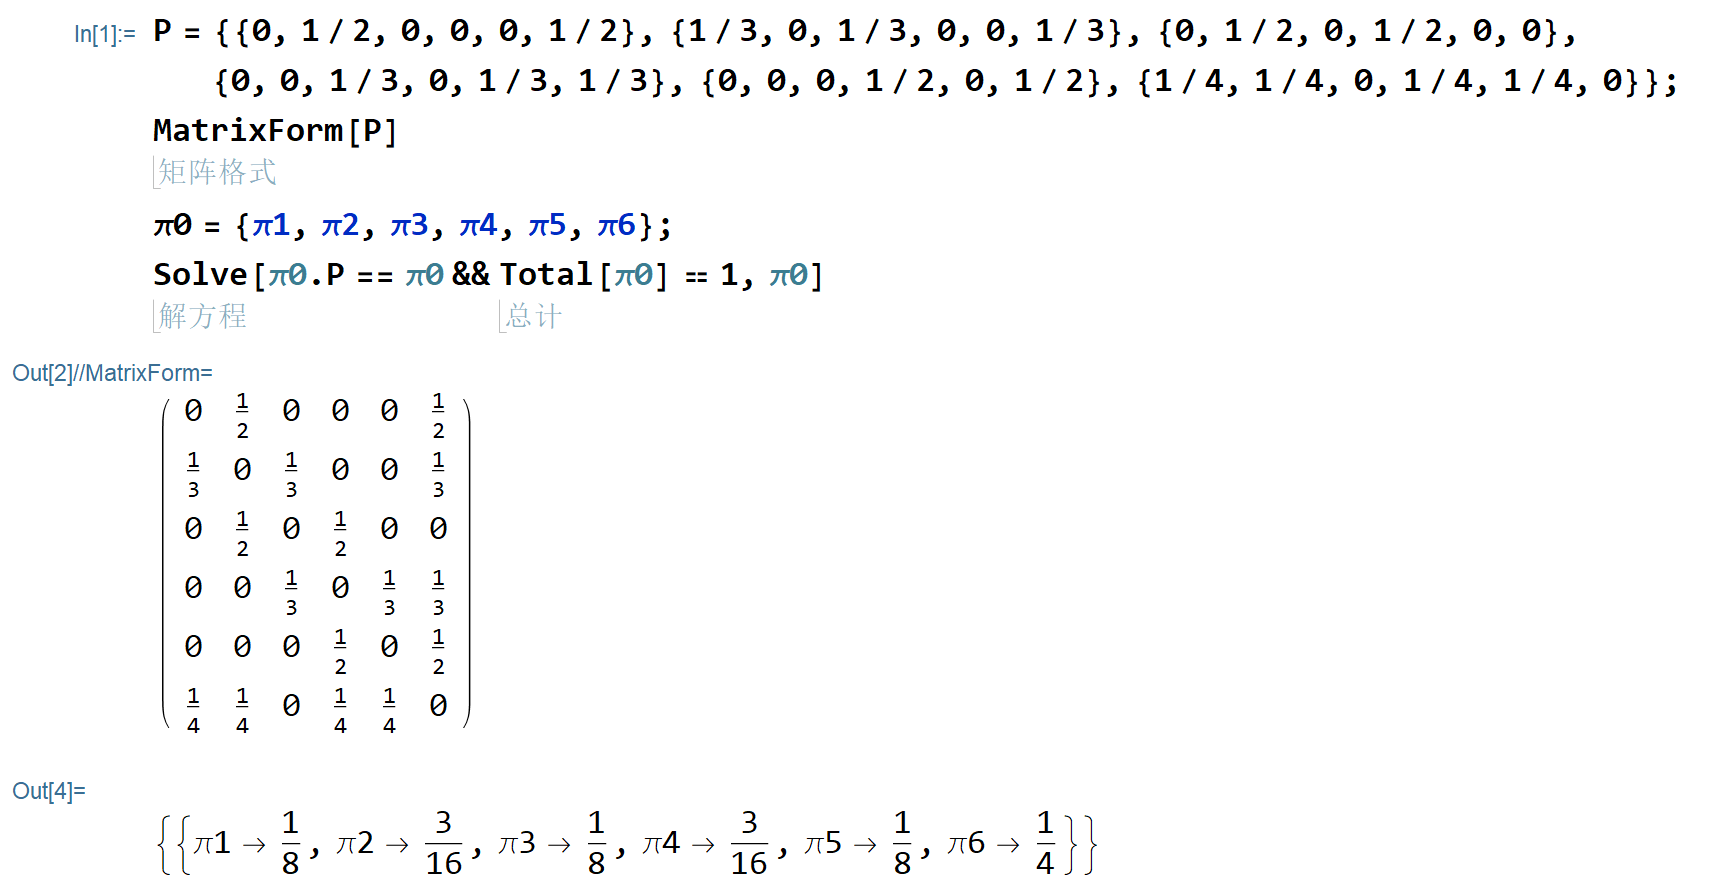
\includegraphics[width=0.9\textwidth]{fig2.png}
			      \caption{利用Mathematica软件验证计算结果}
		      \end{center}\end{figure}


	\item 考察某一系统运作情况(如机器运转)。如果运作正常,则认为系统处于状态1;如果系统正在调整(例如机器维修,计算机杀毒等),则认为系统处于状态0。系统运作一段时间后,会遇到不能正常运作的情况,此时系统需要调整。调整后又恢复运作。假定系统从开始运作直到需要调整的运作时间是随机的,服从参数为\(\mu\)的指数分布,密度函数为\(\mu e^{-\mu t},t>0\)。而调整期也是随机的,服从参数为\(\lambda\)的指数分布,密度函数为\(\lambda e^{-\lambda t},t>0\)。假定运作周期是相互独立的,调整期也是相互独立的。如果令\(X(t)\)为系统在时刻\(t\)所处的状态,则由于在时刻\(t\)以后,系统所处的状态仅与在时刻\(t\)及其以后的剩余运作时间或剩余调整时间有关。利用指数分布的无记忆性知道,\(X(t)\)是时齐Markov链。利用Kolmogorov方程求出此Markov链的转移概率。

	      \begin{align*}
		      p_{01}(\Delta t) & =\int_{0}^{\Delta t}\lambda e^{-\lambda t}dt=1-e^{-\lambda \Delta t}=\lambda \Delta t+o(\Delta t) \\
		      q_{01}           & =\lim_{\Delta t \to 0}\frac{p_{01}(\Delta t)}{\Delta t}=\lambda                                   \\
		      p_{00}(\Delta t) & =1-p_{01}(\Delta t)=1-\lambda \Delta t+o(\Delta t)                                                \\
		      q_{00}           & =\lim_{\Delta t \to 0}\frac{1-p_{01}(\Delta t)}{\Delta t}=\lambda
	      \end{align*}
	      同理可得\(q_{10}=\mu,q_{11}=\mu\)
	      \begin{align*}
		      p_{00}^{\prime}(t)
		       & =-q_{00}p_{00}(t)+q_{10}p_{01}(t)    \\
		       & =-\lambda p_{00}(t)+\mu p_{01}(t)    \\
		       & =-\lambda p_{00}(t)+\mu(1-p_{00}(t)) \\
		       & =-(\lambda+\mu)p_{00}(t)+\mu
	      \end{align*}
	      结合\(p_{00}(0)=1\),解得\(p_{00}(t)=\frac{\mu}{\lambda+\mu}+\frac{\lambda}{\lambda+\mu}e^{-(\lambda+\mu)t}\)
	      \begin{align*}
		      p_{11}^{\prime}
		       & =q_{01}p_{10}(t)-q_{11}p_{11}(t)    \\
		       & =\lambda(1-p_{11}(t))-\mu p_{11}(t) \\
		       & =-(\lambda+\mu)p_{00}(t)+\lambda
	      \end{align*}
	      结合\(p_{11}(0)=1\),解得\(p_{11}(t)=\frac{\lambda}{\lambda+\mu}+\frac{\mu}{\lambda+\mu}e^{-(\lambda+\mu)t}\)。
	\item 设今日有雨,则明日也有雨的概率为0.7,今日无雨,明日有雨的概率为0.5。求星期一有雨,星期三也有雨的概率。

	      记有雨的状态为1,无雨的状态为0。则一步状态转移矩阵为
	      \begin{align*}
		      \mathbf{P}^{(1)}=
		      \begin{pmatrix}
			      0.5 & 0.5 \\
			      0.3 & 0.7
		      \end{pmatrix}
	      \end{align*}
	      则两步转移矩阵为
	      \begin{align*}
		      \mathbf{P}^{(2)}=
		      \begin{pmatrix}
			      0.5 & 0.5 \\
			      0.3 & 0.7
		      \end{pmatrix}^2
		      =\begin{pmatrix}
			       0.4  & 0.5  \\
			       0.36 & 0.64
		       \end{pmatrix}
	      \end{align*}
	      所以\(P\{\)星期一有雨,星期三也有雨\(\}=p^{(2)}_{11}=0.64\)。

	\item 某人有\(r\)把伞用于上下班,如果一天的开始他在家(一天的结束他在办公室)中而且天下雨,只要有伞可取到,他将拿一把到办公室(家)中。如果天不下雨,那么他不带伞,假设每天的开始(结束)下雨的概率为\(p\),不下雨的概率为\(q\),且与过去情况独立。
	      \begin{itemize}[\bfseries (1)]
		      \item 定义一个有\(r+1\)个状态的Markov链并确定转移概率;
		      \item 计算极限分布;
		      \item 他被淋湿的平均次数所占比率是多少?(如果天下雨而全部伞在另一处,那么称他被淋湿)。
	      \end{itemize}

	      \textbf{解答:}\begin{enumerate}[\bfseries (1)]
		      \item 以\(X_n\)表示第\(n\)天此人身边的雨伞数,则\(\{X_n,n=0,1,\ldots \}\)构成一个状态空间为\(\{0,1,2,\cdots ,r\}\)的时齐Markov链。

		            若此人没身边没有伞,所有的\(r\)把伞都在另一个地方,无论是否下雨,他都不会带伞到另一个地方,所以\(p_{0,r}^{(1)}=1\);
		            若此人身边有\(i\)把伞\(0<i\leqslant r\),若不下雨,他不会带伞到另一个地方,所以\(p_{i,r-i}^{(1)}=q\),若下雨,他会带一把伞到另一个地方,所以\(p_{i,r-i+1}^{(1)}=p\)。

		      \item 根据(1),得到一步状态转移矩阵为
		            \begin{align*}
			            \mathbf{P}^{(1)}=\begin{pmatrix}
				                             0      & 0      & 0      & \cdots                                   & 0      & 0      & 1      \\
				                             0      & 0      & 0      & \cdots                                   & 0      & q      & p      \\
				                             0      & 0      & 0      & \cdots                                   & q      & p      & 0      \\
				                             \vdots & \vdots & \vdots & \begin{sideways}\(\ddots\)\end{sideways} & \vdots & \vdots & \vdots \\
				                             0      & 0      & q      & \cdots                                   & 0      & 0      & 0      \\
				                             0      & q      & p      & \cdots                                   & 0      & 0      & 0      \\
				                             q      & p      & 0      & \cdots                                   & 0      & 0      & 0
			                             \end{pmatrix}
		            \end{align*}
		            平稳方程为\begin{align*}
			            \left\{\begin{matrix}
				                   \pi_0=\pi_r q                                         \\
				                   \pi_j=\pi_{r-j}p+\pi_{r-j+1}q,\quad  j=1,2,\ldots,r-1 \\
				                   \pi_r=\pi_0+\pi_1p
			                   \end{matrix}\right.
		            \end{align*}
		            规范性条件为\(\sum_{i=0}^{r}\pi_i=1\)。

		            注意到状态\(j=1,2,\ldots,r-1\)的转移规律相同,所以其极限概率\(\pi_j(j=1,2,\ldots,r-1)\)相等。所以有\(\pi_0=\pi_r q,\pi_0+r\pi_r=1\)。
		            解得
		            \begin{align*}
			            \pi_0 & =\frac{q}{r+q}                      \\
			            \pi_j & =\frac{1}{r+q},\quad j=1,2,\ldots,r
		            \end{align*}
		      \item P\{此人被淋湿\}=P\{此人身边雨伞数为0,下雨\}=P\{此人身边雨伞数为0\}\(\cdot\)P\{下雨\}\(=\pi_0p=\frac{pq}{r+q}\)。

	      \end{enumerate}
	\item 若\(f_{ii}<1,f_{jj}<1\),证明
	      \begin{align*}
		       & \sum_{n=1}^{\infty}p_{ij}^{(n)}<+\infty                                            \\
		       & f_{ij}  =\frac{\sum_{n=1}^{\infty}p_{ij}^{(n)}}{1+\sum_{n=1}^{\infty}p_{jj}^{(n)}}
	      \end{align*}

	      由\(f_{ii}<1,f_{jj}<1\)知,状态\(i,j\)都为非常返状态,所以\(\sum_{n=1}^{\infty}p_{ii}^{(n)}=\frac{1}{1-f_{ii}}\),\(\sum_{n=1}^{\infty}p_{jj}^{(n)}=\frac{1}{1-f_jj}\)。
	      根据转移概率的首达分解定理:
	      \begin{align*}
		      p^{(n)}_{ij}
		       & =\sum_{l=1}^{\infty}f_{ij}^{(l)}p_{jj}^{(n-l)} \\
	      \end{align*}
	      \begin{align*}
		      \sum_{n=1}^{\infty}p_{ij}^{(n)}
		       & =\sum_{n=1}^{\infty}\sum_{l=1}^{\infty}f_{ij}^{(l)}p_{jj}^{(n-l)} \\
		       & =\sum_{l=1}^{\infty}f_{ij}^{(l)}\sum_{n=l}^{\infty}p_{jj}^{(n-l)} \\
		       & =\sum_{l=1}^{\infty}f_{ij}^{(l)}\sum_{m=0}^{\infty}p_{jj}^{(m)}   \\
		       & =f_{ij}\sum_{m=0}^{\infty}p_{jj}^{(m)}                            \\
		       & =f_{ij}+f_{ij}\sum_{m=1}^{\infty}p_{jj}^{(m)}
	      \end{align*}
	      整理得到\(f_{ij}=\frac{\sum_{n=1}^{\infty}p_{ij}^{(n)}}{1-\sum_{n=1}^{\infty}p_{jj}^{(n)}}\)。
	\item 考虑有两个状态的连续时间Markov链,状态为0和1,链在离开0到达1之前在状态0停留的时间服从参数为\(\lambda\)的指数分布,相应地在1停留的时间是参数为\(\mu\)的指数变量。对此建立Markov微分方程,并求其解。

	      \textbf{同第(2)题}
	\item 设有一质点在1,2,3上做随机跳跃,在时刻t它位于三点之一,且在\([t,t+h]\)内以概率\(\frac{1}{2}+o(h)\)分别可以跳到其他两个状态。试求状态概率满足的Kolmogorov方程。

	      记X为质点所处状态,\(P\{x(t+h)=2|X(t)=1\}=P\{x(t+h)=3|X(t)=1\}=\frac{h}{2}+o(h)\),\(P\{x(t+h)=1|X(t)=1\}=1-h+0(h)\),
	      可以求得
	      \begin{align*}
		      q_{21}=q_{31}
		       & =\lim_{h\to 0}\frac{p_{i1}(t)}{h}        \\
		       & =\lim_{h\to 0}\frac{\frac{h}{2}+o(h)}{h} \\
		       & =\frac{1}{2}                             \\
		      q_{11}
		       & =\lim_{h\to 0}\frac{1-p_{11}(h)}{h}      \\
		       & =\lim_{h\to 0}\frac{1-(1-h+o(h))}{h}     \\
		       & =1
	      \end{align*}
	      利用Kolmogorov前向方程:
	      \begin{align*}
		      p^{\prime}_{12}(t)
		       & =q_{32}p_{13}(t)+q_{12}p_{11}(t)-q_{22}p_{12}(t)     \\
		       & =\frac{1}{2}p_{13}(t)+\frac{1}{2}p_{11}(t)-p_{12}(t) \\
		       & =\frac{1}{2}(1-p_{12}(t))-p_{12}(t)                  \\
		       & =-\frac{3}{2}p_{12}(t)+\frac{1}{2}
	      \end{align*}
	      结合\(p_{12}(0)=0\)解得,\(p_{12}(t)=\frac{1-e^{-3t/2}}{3}\)。同理得\(p_{13}(t)=\frac{1-e^{-3t/2}}{3},p_{11}(t)=1-p_{12}(t)-p_{13}(t)=\frac{2e^{-3t/2}+1}{3}\)。
\end{enumerate}

\section{鞅}

\begin{enumerate}
	\item 设\(Y_0,Y_1,Y_2,\cdots\)是一系列独立随机变量且\(E\lvert Y_n\rvert<+\infty,EY_n=0\)。令\(X_n=\sum_{i=0}^{n}Y_i,n=0,1,2,\cdots,\mathscr{F}_n=\sigma\{Y_i,i=0,1,2,\cdots,n\}\),则\(\{X_n,\mathscr{F}_n\}\)是一个鞅。

	      \textbf{证明}:由于\(X_n=\sum_{i=0}^{n}Y_i,n=0,1,2,\cdots\),显然\(X_n\)是\(\sigma\{Y_i,i=0,1,2,\cdots,n\}\)可测的。
	      \begin{align*}
		      E|X_n|\leqslant \sum_{n=0}^{n}|Y_i|<+\infty
	      \end{align*}
	      且
	      \begin{align*}
		      E[X_{n+1}|Y_0,Y_1,\cdots,Y_n]
		       & =E[X_n+Y_{n+1}|Y_0,Y_1,\cdots,Y_n]                       \\
		       & =E[X_n|Y_0,Y_1,\cdots,Y_n]+E[Y_{n+1}|Y_0,Y_1,\cdots,Y_n] \\
		       & =X_n+E[Y_n]                                              \\
		       & =X_n
	      \end{align*}
	      所以\(\{X_n,\mathscr{F}_n\}\)是一个鞅。
	\item 设\(Y_0,Y_1,Y_2,\ldots ,Y_n\)如上题假定,另外设\(EY^2_n=\sigma^2,n=1,2,\ldots,\)令\(Z_0=0,Z_n=\left(\sum_{i=1}^{n}Y_i\right)^2-n\sigma^2\),那么\(\{Z_n,\mathscr{F}_n\}\)是一个鞅。

	      \textbf{证明}:由于\(Z_n=(\sum_{i=0}^{n}Y_i)^2-n\sigma^2,n=0,1,2,\cdots\),显然\(Z_n\)是\(\sigma\{Y_i,i=0,1,2,\cdots,n\}\)可测的。
	      \begin{align*}
		      E|Z_n|=E|(\sum_{i=0}^{n}Y_i)^2-n\sigma^2|\leqslant2n\sigma^2<+\infty
	      \end{align*}
	      \begin{align*}
		        & E[Z_{n+1}|Y_0,Y_1,\cdots,Y_n]                                                                      \\
		      = & E[(\sum_{i=0}^{n+1}Y_i)^2-(n+1)\sigma^2|Y_0,Y,1,\cdots,Y_n]                                        \\
		      = & E[(\sum_{i=0}^{n}Y_i+Y_{n+1})^2-(n+1)\sigma^2|Y_0,Y,1,\cdots,Y_n]                                  \\
		      = & E[(\sum_{i=0}^{n}Y_i)^2+Y_{n+1}^2+2Y_{n+1}\sum_{i=0}^{n}Y_i-(n+1)\sigma^2|Y_0,Y,1,\cdots,Y_n]      \\
		      = & E[(\sum_{i=0}^{n}Y_i)^2-n\sigma^2+Y_{n+1}^2-\sigma^2+2Y_{n+1}\sum_{i=0}^{n}Y_i|Y_0,Y,1,\cdots,Y_n] \\
		      = & E[(\sum_{i=0}^{n}Y_i)^2-n\sigma^2|Y_0,Y,1,\cdots,Y_n]+E[Y_{n+1}^2-\sigma^2|Y_0,Y,1,\cdots,Y_n]     \\
		        & +E[2Y_{n+1}\sum_{i=0}^{n}Y_i|Y_0,Y,1,\cdots,Y_n]                                                   \\
		      = & E[Y_{n+1}^2-\sigma^2]+2E[Y_{n+1}]\sum_{i=0}^{n}Y_i+(\sum_{i=0}^{n}Y_i)^2-n\sigma^2                 \\
		      = & Z_n
	      \end{align*}
	      所以\(\{Z_n,\mathscr{F}_n\}\)是一个鞅。
	\item 令\(X_0,X_1,\cdots\)表示分支过程各代的个体数,\(X_0=1\),任意一个个体生育后代的分布有均值\(\mu\)。证明\(\{M_n=\mu^{-n}X_n\}\)是一个关于\(X_0,X_1,\cdots\)的鞅。

	      \textbf{证明:}由于\(M_n=\mu^{-n}X_n,n=0,1,2,\cdots\),显然\(M_n\)是\(\sigma\{X_i,i=0,1,2,\cdots,n\}\)可测的。
	      \begin{align*}
		      E|M_n|=E|X_n|\mu^{-n}=\mu^{n}\mu^{-n}=1<\infty
	      \end{align*}
	      \begin{align*}
		      E[M_{n+1}|X_0,X_1,\cdots,X_n]
		       & =E[\mu^{-n-1}X_{n+1}|X_0,X_1,\cdots,X_n] \\
		       & =\mu^{-n-1}E[X_{n+1}|X_0,X_1,\cdots,X_n] \\
		       & =\mu^{-n-1}E[X_{n+1}|X_n]                \\
		       & =\mu^{-n-1}\cdot \mu X_n                 \\
		       & =\mu^{n}X_n                              \\
		       & =M_n
	      \end{align*}
	      所以\(\{M_n=\mu^{-n}X_n\}\)是一个关于\(X_0,X_1,\cdots\)的鞅。
	\item 考虑一个在整数上的随机游动模型,设向右移动的概率\(p<\frac{1}{2}\),向左移动的概率为\(1-p,S_n\)表示时刻n所处的位置,假定\(S_0=a,0<a<N\)。
	      \begin{itemize}[\bfseries (1)]
		      \item 证明:\(\{M_n=\left(\frac{1-p}{p}\right)^{S_n}\}\)是鞅;
		      \item 令T表示随机游动第一次到达0或N的时刻,即
		            \begin{align*}
			            T=\min\{n:S_n=0orN\}
		            \end{align*}
		            利用鞅停时定理,求出\(P\{S_T=0\}\)。
	      \end{itemize}

	      \begin{enumerate}[\bfseries (1)]
		      \item \textbf{证明:}易知\(\{M_n\}\)关于\(\sigma(S_0,S_1,\cdots,S_n)\)可测的。
		            \begin{align*}
			            E|M_n|
			             & =E\bigg|\left(\frac{1-p}{p}\right)^{S_n}\bigg|                             \\
			             & =E\left[\frac{1-p}{p}\right]^{S_n}                                         \\
			             & \leqslant\left(\max\left\{\frac{1-p}{p},\frac{p}{1-p}\right\}\right)^{a+n} \\
			             & <+\infty
		            \end{align*}
		            \begin{align*}
			            E & [M_{n+1}|S_0,S_1,\ldots,S_n]                                                      \\
			              & =E\left[\bigg(\frac{1-p}{p}\bigg)^{S_{n+1}}|S_0,S_1,\ldots,S_n\right]             \\
			              & =E\left[\bigg(\frac{1-p}{p}\bigg)^{S_n}\bigg(\frac{1-p}{p}\bigg)^{X_{n+1}}
			            |S_0,S_1,\ldots,S_n\right]                                                            \\
			              & =\bigg(\frac{1-p}{p}\bigg)^{S_n}
			            E\left[\bigg(\frac{1-p}{p}\bigg)^{X_{n+1}}|S_0,S_1,\ldots,S_n\right]                  \\
			              & =\bigg(\frac{1-p}{p}\bigg)^{S_n}E\left[\bigg(\frac{1-p}{p}\bigg)^{X_{n+1}}\right] \\
			              & =\bigg(\frac{1-p}{p}\bigg)^{S_n}(\frac{1-p}{p}\cdot p+\frac{p}{1-p}\cdot (1-p))   \\
			              & =\bigg(\frac{1-p}{p}\bigg)^{S_n}                                                  \\
			              & =M_n
		            \end{align*}
		            所以\(\{M_n=\left(\frac{1-p}{p}\right)^{S_n}\}\)是关于\(\{S_0\}\)鞅。
		      \item 显然T是关于\(\{M_n,n=0,1,2,\ldots,\}\)的停时,并且由(1)知\(\{M_n<+\infty\}\),若\(P\{T<\infty\}=1\),由停时定理
		            \begin{align*}
			            E(M_T)=E(M_0)=\bigg(\frac{1-p}{p}\bigg)^a
		            \end{align*}
		            即
		            \begin{align*}
			            E[M_T]  & =1\times P\{M_T=1\}+\bigg(\frac{1-p}{p} \bigg)\times P\{S_T=N\} \\
			            =E[M_0] & =\bigg(\frac{1-p}{p}\bigg)^a
		            \end{align*}
		            并且\begin{align*}
			            P\{S_T=0\}+P\{S_T=N\}=1
		            \end{align*}
		            解得
		            \begin{align*}
			            P{S_T=0}
			             & =\frac{(\frac{1-p}{p})^a-(\frac{1-p}{p})^N}{1-(\frac{1-p}{p})^N} \\
			             & =\frac{p^N(1-p)^a-p^a(1-p)^N}{p^{N+a}-p^a(1-p)^N}
		            \end{align*}
	      \end{enumerate}
\end{enumerate}


\section{Brown运动}

\begin{enumerate}
	\item 设\(\{B(t),t\geqslant0\}\)是标准Brown运动,计算\(P\{B(2)\leqslant0\}\)和\(P\{B(t),\leqslant0,t=0,1,2\)\}。

	      \(B(2)\sim \mathcal{N}(0,2)\),由正态分布函数的对称性可知\(P\{B(2)\leqslant0\}=1/2\)。

	      \begin{align*}
		      P\{B(t)\leqslant 0,\leqslant0,t=0,1,2\}
		       & =P\{B(1)\leqslant0,B(2)\leqslant0\}                \\
		       & =P\{B(1)\leqslant0,B(1)+B(2)-B(1)\leqslant0\}      \\
		       & =\int_{-\infty}^{0}P\{B(2)-B(1)\leqslant-x\}f(x)dx \\
		       & =\int_{-\infty}^{\infty}\Phi(-x)d\Phi(x)           \\
		       & =3/8
	      \end{align*}
	\item 设\(\{B(t)\}\)是Brown运动,求\(B(1)+B(2)+B(3)+B(4)\)的分布。
	      对于标准Brown运动\(B(t)\sim \mathcal{N}(0,t)\)。
	      \begin{align*}
		      B & (1)+B(2)+B(3)+B(4)                         \\
		        & =4B(1)+3(B(2)-B(1))+2(B(3)-B(2))+B(4)-B(3) \\
		        & \sim \mathcal{N}(0,4^2+3^2+2^2+1)          \\
		        & =\mathcal{N}(0,30)
	      \end{align*}
	\item 求\(B(\frac{1}{4})+B(\frac{1}{2})+B(\frac{3}{4})+B(1)\)的分布。
	      \begin{align*}
		      B & (1/4)+B(1/2)+B(3/4)+B(1)                               \\
		        & =4B(1/4)+3(B(1/2)-B(1/4))+2(B(3/4)-B(1/2))+B(1)-B(3/4) \\
		        & \sim \mathcal{N}(0,\frac{4^2+3^2+2^2+1}{4})            \\
		        & =\mathcal{N}(0,\frac{15}{2})
	      \end{align*}
	\item 求概率\(P\{\int_{0}^{1} B(t)dt>\frac{2}{\sqrt{3}}\}\)。
	      \begin{align*}
		      Var\left[\int_{0}^{1} B(t)dt\right]
		       & =Cov\left[\int_{0}^{1} B(t)dt,\int_{0}^{1} B(s)ds\right]     \\
		       & =E\left[\int_{0}^{1} B(t)dt\int_{0}^{1} B(s)ds\right]        \\
		       & =\int_{0}^{1}\int_{0}^{1}E[B(t)B(s)]dtds                     \\
		       & =\int_{0}^{1}\int_{0}^{1}Cov[B(t)B(s)]dtds                   \\
		       & =\int_{0}^{1}\min\{t,s\}dtds                                 \\
		       & =\int_{0}^{1}dt\int_{0}^{t}sds+\int_{0}^{1}ds\int_{0}^{s}tdt \\
		       & =\frac{1}{2}\int_{0}^{1}t^2dt+\frac{1}{2}\int_{0}^{1}s^2ds   \\
		       & =1/3
	      \end{align*}
	      所以\(\int_{0}^{1}B(t)dt\sim \mathcal{N}(0,1/3)\),所求概率为
	      \begin{align*}
		      P\{\int_{0}^{1}B(t)dt>\frac{2}{\sqrt{3}}\}
		       & =P\{\sqrt{3}\int_{0}^{1}B(t)dt>2\} \\
		       & =1-\Phi(2)                         \\
		       & \approx 0.023
	      \end{align*}
	\item 设\(\{B(t),t\geqslant0\}\)为标准Brown运动,求\(B(1)+B(2)+\cdots+B(n)\)的分布,并验证\(\{X(t)-tB(\frac{1}{t})\}\)仍为\([0,+\infty)\)上的Brown运动。

	      \begin{align*}
		      B(1) & +B(2)+\cdots+B(n)                                           \\
		           & =nB(1)+(n-1)(B(2)-B(1))+\cdots+2(B(n-1)-B(n-2))+B(n)-B(n-1) \\
		           & \sim\mathcal{N}(0,\sum_{i=1}^{n}n^2)                        \\
		           & =\mathcal{N}(0,\frac{n(n+1)(2n+1)}{6})
	      \end{align*}

	      由于\(X(t)=tB(\frac{1}{t})\),所以\(X(0)=0\)(?)

	      \(\forall 0<s<t<+\infty\)
	      \begin{align*}
		        & X(t)-X(s)                                                                \\
		      = & tB\bigg(\frac{1}{t}\bigg)-sB\bigg(\frac{1}{s}\bigg)                      \\
		      = & tB\bigg(\frac{1}{t}\bigg)-sB\bigg(\frac{1}{t}\bigg)
		      +sB\bigg(\frac{1}{t}\bigg)-sB\bigg(\frac{1}{s}\bigg)                         \\
		      = & (t-s)B\bigg(\frac{1}{t}\bigg)-s\bigg[B(\frac{1}{t})-B(\frac{1}{s})\bigg]
	      \end{align*}
	      由于\(\{B(t),t\geqslant0\}\)是标准Brown运动,所以\(X(t)-X(s)\)服从正态分布,
	      \begin{align*}
		       & E[X(t)-X(s)]=0                                                     \\
		       & Var[X(t)-X(s)]=(t-s)^2\frac{1}{t}+s^2(\frac{1}{s}-\frac{1}{t})=t-s
	      \end{align*}
	      所以\(X(t)-X(s)\sim \mathcal{N}(0,t-s)\),所以\(\{X(t),t\geqslant0\}\)是标准Brown运动。
\end{enumerate}

\section{随机积分}

\begin{enumerate}
	\item 求\(d(e^{B(t)})\)。
	      \begin{align*}
		      dB(t)=\mu(t)dt+\sigma(t)dW(t)
	      \end{align*}
	      \begin{align*}
		      d(e^{B(t)}) & =e^{B(t)}dB(t)+\frac{1}{2}e^{B(t)}dB(t)^2                \\
		                  & =e^{B(t)}(\mu(t)dt+\sigma(t)dW(t))+\frac{1}{2}e^{B(t)}dt \\
		                  & =e^{B(t)}(\mu(t)+\frac{1}{2})dt+e^{B(t)}dW(t)
	      \end{align*}
	\item 求解Ornstein-Uhlenbeck方程\begin{align*}dX_t=-\mu X_tdt+\sigma dB_t\end{align*}其中\(\mu,\sigma\)为常数。
	      \begin{align*}
		      \frac{d}{dt}[e^{\mu t}X(t)]
		       & =\mu e^{\mu t}X(t)dt+e^{\mu t}dX(t) \\
		       & =e^{\mu t}\sigma dB(t)
	      \end{align*}
	      等式两边积分得到
	      \begin{align*}
		      e^{\mu t}X(t)\bigg|^t_{t_0}=\int_{t_0}^{t}e^{\mu s}dB(s)
	      \end{align*}
	      整理得到
	      \begin{align*}
		      X(t)=X(t_0)e^{\mu (t_0-t)}+e^{-\mu t}\int_{t_0}^{t}e^{\mu s}dB(s)
	      \end{align*}
	\item 考虑群体增长模型
	      \begin{align*}
		      \frac{dN_t}{dt}=a_tN_t
	      \end{align*}其
	      中\(N_0\)已知,\(a_t=r_t+\alpha B_t\),\(r_t\)为增长率(假设为常数\(r\)),\(\alpha\)为常数,\(B_t\)为Brown运动。
	      可以将其化为随机微分方程的形式。
	      \begin{align*}
		      dN_t=rN_tdt+\alpha N_tdB_t
	      \end{align*}
	      这种类型的方程被称为集合随机微分方程,试求解它。

	      \textbf{解答:}由题意得到
	      \begin{align*}
		      \frac{dN_t}{N_t}=rdt+\alpha dB_t
	      \end{align*}
	      则
	      \begin{align*}
		      d\ln N_t & =\frac{1}{N_t}dN_t-\frac{1}{2}\frac{1}{N_t^2}dN_t^2  \\
		               & =rdt+\alpha dB_t-\frac{(\alpha N_t)^2dB_t^2}{2N_t^2} \\
		               & =(r-\frac{\alpha^2}{2})dt+\alpha dB_t
	      \end{align*}
	      等式两端积分得到
	      \begin{align*}
		      \ln N_t-\ln N_0=(r-\frac{\alpha^2}{2})t+\alpha B_t
	      \end{align*}
	      其中用到了\(B(0)=0\)。整理得到
	      \begin{align*}
		      N_t=N_0\exp \left[(r-\frac{\alpha^2}{2})t+\alpha B_t \right]
	      \end{align*}
	\item 设\(X(t)\)具有随机微分形式
	      \begin{align*}
		      dX(t)=(bX(t)+c)dt+2\sqrt{X(t)}dB(t)
	      \end{align*}
	      并假定\(X(t)\geqslant0\),试找出过程\(\{Y(t)=\sqrt{X(t)}\}\)的随机微分形式。

	      \begin{align*}
		      dY(t) & =\frac{1}{2}\frac{1}{\sqrt{X(t)}}dX(t)-\frac{1}{2}\frac{1}{4X^{3/2}(t)}dX^2(t)       \\
		            & =\frac{(bX(t)+c)dt+2\sqrt{X(t)}dB(t)}{2\sqrt{X(t)}}-\frac{4X(t)dB^2(t)}{8X^{3/2}(t)} \\
		            & =\frac{b}{2}\sqrt{X(t)}dt+\frac{c}{2\sqrt{X(t)}}dt+dB(t)-\frac{dt}{2\sqrt{X(t)}}     \\
		            & =(\frac{b}{2}\sqrt{X(t)}+\frac{c+1}{2\sqrt{X(t)}})dt+dB(t)                           \\
		            & =(\frac{b}{2}Y(t)+\frac{c+1}{2Y(t)})dt+dB(t)
	      \end{align*}
	      即所求随机微分形式为\(dY(t)=(\frac{b}{2}Y(t)+\frac{c+1}{2Y(t)})dt+dB(t)\)。
	\item 利用It\(\hat{o}\)公式证明
	      \begin{align*}
		      \int_{0}^{t}B^2(s)ds=\frac{1}{3}B^3(t)-\int_{0}^{t}B(s)ds
	      \end{align*}

	      \textbf{证明:}利用It\(\hat{o}\)公式
	      \begin{align*}
		      d(B^3(t))
		       & =\frac{\partial}{\partial t}B^3(t)dt+\frac{1}{2}\frac{\partial^2}{\partial t^2}B^3(t)dB^2(t) \\
		       & =3B^2(t)dt+\frac{6B(t)}{2}dB^2(t)                                                            \\
		       & =3B^2(t)dt+3B(t)dt
	      \end{align*}
	      等式两端积分得到
	      \begin{align*}
		      B^3(s)\bigg|_0^t=3\int_{0}^{t}B^2(s)ds+3\int_{0}^{t}B(s)dB(s)
	      \end{align*}
	      利用\(B(0)=0\),整理得到
	      \begin{align*}
		      \int_{0}^{t}B^2(s)=\frac{1}{3}B^3(t)-\int_{0}^{t}B(s)ds
	      \end{align*}
	\item 设\(\{X(t),Y(t)\}\)是It\(\hat{o}\)过程,试证
	      \begin{align*}
		      d(X(t)Y(t))=X(t)dY(t)+Y(t)dX(t)+dX(t)\cdot dY(t)
	      \end{align*}
	      由此导出下面的分部积分公式
	      \begin{align*}
		      \int_{0}^{t}X(s)dY(s)=X(t)Y(t)-X(0)Y(0)-\int_{0}^{t}Y(s)dX(s)-\int_{0}^{t}dX(s)\cdot dY(s)
	      \end{align*}

	      \textbf{证明:}
	      \begin{align*}
		      d(X(t)                       & Y(t))                                                              \\
		      =\frac{\partial}{\partial t} & (X(t)Y(t))dt+\frac{\partial(X(t)Y(t))}{\partial X(t)}dX(t)
		      +\frac{\partial(X(t)Y(t))}{\partial Y(t)}dY(t)                                                    \\
		                                   & +\frac{1}{2}\frac{\partial^2(X(t)Y(t))}{\partial X^2(t)}dX^2(t)
		      +\frac{1}{2}\frac{\partial^2(X(t)Y(t))}{\partial Y^2(t)}dY^2(t)                                   \\
		                                   & +\frac{\partial^2(X(t)Y(t))}{\partial X(t)\partial Y(t)}dX(t)dY(t) \\
		      =Y(t)                        & dX(t)+X(t)dY(t)+dX(t)\cdot dY(t)
	      \end{align*}
\end{enumerate}

% 如有附录则在以下引入
% \appendix

%\backmatter
% 使用 bibLaTeX 制作书目
\printbibliography[heading=bibintoc]


% 制作索引: 先是符号索引, 继而是名词索引暨英译
{\footnotesize
	\printindex[sym1]
	\indexprologue{中文术语按汉语拼音排序.}
	\printindex
	%	如有需要, 加入表格和图片索引
	%	\cleardoublepage
	% 	\phantomsection
	%	\addcontentsline{toc}{chapter}{\listfigurename}
	%	\listoffigures
	%	\cleardoublepage
	% 	\phantomsection
	%	\addcontentsline{toc}{chapter}{\listtablename}
	%	\listoftables
}
\end{document}